% Options for packages loaded elsewhere
\PassOptionsToPackage{unicode}{hyperref}
\PassOptionsToPackage{hyphens}{url}
%
\documentclass[
]{book}
\title{PSYC753 Data Fluency: Analysis}
\author{Chris Berry}
\date{}

\usepackage{amsmath,amssymb}
\usepackage{lmodern}
\usepackage{iftex}
\ifPDFTeX
  \usepackage[T1]{fontenc}
  \usepackage[utf8]{inputenc}
  \usepackage{textcomp} % provide euro and other symbols
\else % if luatex or xetex
  \usepackage{unicode-math}
  \defaultfontfeatures{Scale=MatchLowercase}
  \defaultfontfeatures[\rmfamily]{Ligatures=TeX,Scale=1}
\fi
% Use upquote if available, for straight quotes in verbatim environments
\IfFileExists{upquote.sty}{\usepackage{upquote}}{}
\IfFileExists{microtype.sty}{% use microtype if available
  \usepackage[]{microtype}
  \UseMicrotypeSet[protrusion]{basicmath} % disable protrusion for tt fonts
}{}
\makeatletter
\@ifundefined{KOMAClassName}{% if non-KOMA class
  \IfFileExists{parskip.sty}{%
    \usepackage{parskip}
  }{% else
    \setlength{\parindent}{0pt}
    \setlength{\parskip}{6pt plus 2pt minus 1pt}}
}{% if KOMA class
  \KOMAoptions{parskip=half}}
\makeatother
\usepackage{xcolor}
\IfFileExists{xurl.sty}{\usepackage{xurl}}{} % add URL line breaks if available
\IfFileExists{bookmark.sty}{\usepackage{bookmark}}{\usepackage{hyperref}}
\hypersetup{
  pdftitle={PSYC753 Data Fluency: Analysis},
  pdfauthor={Chris Berry},
  hidelinks,
  pdfcreator={LaTeX via pandoc}}
\urlstyle{same} % disable monospaced font for URLs
\usepackage{color}
\usepackage{fancyvrb}
\newcommand{\VerbBar}{|}
\newcommand{\VERB}{\Verb[commandchars=\\\{\}]}
\DefineVerbatimEnvironment{Highlighting}{Verbatim}{commandchars=\\\{\}}
% Add ',fontsize=\small' for more characters per line
\usepackage{framed}
\definecolor{shadecolor}{RGB}{248,248,248}
\newenvironment{Shaded}{\begin{snugshade}}{\end{snugshade}}
\newcommand{\AlertTok}[1]{\textcolor[rgb]{0.94,0.16,0.16}{#1}}
\newcommand{\AnnotationTok}[1]{\textcolor[rgb]{0.56,0.35,0.01}{\textbf{\textit{#1}}}}
\newcommand{\AttributeTok}[1]{\textcolor[rgb]{0.77,0.63,0.00}{#1}}
\newcommand{\BaseNTok}[1]{\textcolor[rgb]{0.00,0.00,0.81}{#1}}
\newcommand{\BuiltInTok}[1]{#1}
\newcommand{\CharTok}[1]{\textcolor[rgb]{0.31,0.60,0.02}{#1}}
\newcommand{\CommentTok}[1]{\textcolor[rgb]{0.56,0.35,0.01}{\textit{#1}}}
\newcommand{\CommentVarTok}[1]{\textcolor[rgb]{0.56,0.35,0.01}{\textbf{\textit{#1}}}}
\newcommand{\ConstantTok}[1]{\textcolor[rgb]{0.00,0.00,0.00}{#1}}
\newcommand{\ControlFlowTok}[1]{\textcolor[rgb]{0.13,0.29,0.53}{\textbf{#1}}}
\newcommand{\DataTypeTok}[1]{\textcolor[rgb]{0.13,0.29,0.53}{#1}}
\newcommand{\DecValTok}[1]{\textcolor[rgb]{0.00,0.00,0.81}{#1}}
\newcommand{\DocumentationTok}[1]{\textcolor[rgb]{0.56,0.35,0.01}{\textbf{\textit{#1}}}}
\newcommand{\ErrorTok}[1]{\textcolor[rgb]{0.64,0.00,0.00}{\textbf{#1}}}
\newcommand{\ExtensionTok}[1]{#1}
\newcommand{\FloatTok}[1]{\textcolor[rgb]{0.00,0.00,0.81}{#1}}
\newcommand{\FunctionTok}[1]{\textcolor[rgb]{0.00,0.00,0.00}{#1}}
\newcommand{\ImportTok}[1]{#1}
\newcommand{\InformationTok}[1]{\textcolor[rgb]{0.56,0.35,0.01}{\textbf{\textit{#1}}}}
\newcommand{\KeywordTok}[1]{\textcolor[rgb]{0.13,0.29,0.53}{\textbf{#1}}}
\newcommand{\NormalTok}[1]{#1}
\newcommand{\OperatorTok}[1]{\textcolor[rgb]{0.81,0.36,0.00}{\textbf{#1}}}
\newcommand{\OtherTok}[1]{\textcolor[rgb]{0.56,0.35,0.01}{#1}}
\newcommand{\PreprocessorTok}[1]{\textcolor[rgb]{0.56,0.35,0.01}{\textit{#1}}}
\newcommand{\RegionMarkerTok}[1]{#1}
\newcommand{\SpecialCharTok}[1]{\textcolor[rgb]{0.00,0.00,0.00}{#1}}
\newcommand{\SpecialStringTok}[1]{\textcolor[rgb]{0.31,0.60,0.02}{#1}}
\newcommand{\StringTok}[1]{\textcolor[rgb]{0.31,0.60,0.02}{#1}}
\newcommand{\VariableTok}[1]{\textcolor[rgb]{0.00,0.00,0.00}{#1}}
\newcommand{\VerbatimStringTok}[1]{\textcolor[rgb]{0.31,0.60,0.02}{#1}}
\newcommand{\WarningTok}[1]{\textcolor[rgb]{0.56,0.35,0.01}{\textbf{\textit{#1}}}}
\usepackage{longtable,booktabs,array}
\usepackage{calc} % for calculating minipage widths
% Correct order of tables after \paragraph or \subparagraph
\usepackage{etoolbox}
\makeatletter
\patchcmd\longtable{\par}{\if@noskipsec\mbox{}\fi\par}{}{}
\makeatother
% Allow footnotes in longtable head/foot
\IfFileExists{footnotehyper.sty}{\usepackage{footnotehyper}}{\usepackage{footnote}}
\makesavenoteenv{longtable}
\usepackage{graphicx}
\makeatletter
\def\maxwidth{\ifdim\Gin@nat@width>\linewidth\linewidth\else\Gin@nat@width\fi}
\def\maxheight{\ifdim\Gin@nat@height>\textheight\textheight\else\Gin@nat@height\fi}
\makeatother
% Scale images if necessary, so that they will not overflow the page
% margins by default, and it is still possible to overwrite the defaults
% using explicit options in \includegraphics[width, height, ...]{}
\setkeys{Gin}{width=\maxwidth,height=\maxheight,keepaspectratio}
% Set default figure placement to htbp
\makeatletter
\def\fps@figure{htbp}
\makeatother
\setlength{\emergencystretch}{3em} % prevent overfull lines
\providecommand{\tightlist}{%
  \setlength{\itemsep}{0pt}\setlength{\parskip}{0pt}}
\setcounter{secnumdepth}{5}
\usepackage{booktabs}

\usepackage{tcolorbox}
\usepackage[T1]{fontenc}

\definecolor{dangcol}{RGB}{152,62,130}
\definecolor{warncol}{RGB}{245,220,112}
\definecolor{infocol}{RGB}{70,122,172}
\definecolor{trycol}{RGB}{97,88,156}

\newtcolorbox{dangerous}{
  colback=dangcol!10,
  colframe=dangcol,
  coltext=black,
  boxsep=5pt,
  arc=4pt
}

\newtcolorbox{warning}{
  colback=warncol!10,
  colframe=warncol,
  coltext=black,
  boxsep=5pt,
  arc=4pt
}

\newtcolorbox{info}{
  colback=infocol!10,
  colframe=infocol,
  coltext=black,
  boxsep=5pt,
  arc=4pt
}

\newtcolorbox{try}{
  colback=trycol!10,
  colframe=trycol,
  coltext=black,
  boxsep=5pt,
  arc=4pt
}
\ifLuaTeX
  \usepackage{selnolig}  % disable illegal ligatures
\fi
\usepackage[]{natbib}
\bibliographystyle{apalike}

\usepackage{amsthm}
\newtheorem{theorem}{Theorem}[chapter]
\newtheorem{lemma}{Lemma}[chapter]
\newtheorem{corollary}{Corollary}[chapter]
\newtheorem{proposition}{Proposition}[chapter]
\newtheorem{conjecture}{Conjecture}[chapter]
\theoremstyle{definition}
\newtheorem{definition}{Definition}[chapter]
\theoremstyle{definition}
\newtheorem{example}{Example}[chapter]
\theoremstyle{definition}
\newtheorem{exercise}{Exercise}[chapter]
\theoremstyle{definition}
\newtheorem{hypothesis}{Hypothesis}[chapter]
\theoremstyle{remark}
\newtheorem*{remark}{Remark}
\newtheorem*{solution}{Solution}
\begin{document}
\maketitle

{
\setcounter{tocdepth}{1}
\tableofcontents
}
\hypertarget{overview}{%
\chapter*{Overview}\label{overview}}
\addcontentsline{toc}{chapter}{Overview}

This workbook contains details of the seven sessions given by \textbf{Chris Berry}:

\begin{itemize}
\item
  17/01/22. Simple regression.
\item
  24/01/22. Multiple regression 1: multiple continuous predictors
\item
  31/01/22. ANOVA 1: one-way
\item
  07/02/22. Multiple regression 2: one continuous, one categorical
\item
  14/02/22. Multiple regression 3: evaluating and comparing models
\item
  21/02/22 - No session
\item
  28/02/22. ANOVA 2: factorial
\item
  07/03/22. Pre-post data, effect sizes, clinically significant change
\end{itemize}

\hfill\break

It also contains details of:

\begin{itemize}
\item
  the Regression \textbf{assessment}
\item
  the assessment FAQs
\end{itemize}

\hfill\break

\hfill\break

\hypertarget{simple-regression}{%
\chapter{Simple Regression}\label{simple-regression}}

\textbf{stuff here}

\hypertarget{multiple1}{%
\chapter{Multiple regression: multiple continuous predictors}\label{multiple1}}

\emph{January 2022}

\hypertarget{in-brief}{%
\subsection{In brief}\label{in-brief}}

\begin{quote}
Models need to be \emph{appropriately complex}. That is, we want to make models
that represent our theories for the underlying causes of our data. Often this
means adding many variables to a regression model. But we won't
always be sure which variables to add. Adding multiple variables also brings
challenges. Where predictors are highly correlated (termed \textbf{multicollinearity})
then model results can be confusing.
\end{quote}

\hypertarget{multiple-regression-with-several-continuous-predictors}{%
\section{Multiple regression with several continuous predictors}\label{multiple-regression-with-several-continuous-predictors}}

\begin{itemize}
\tightlist
\item
  \href{slides/PSYC753_Chris1.pptx}{Slides for the session}
\end{itemize}

\hypertarget{overview-1}{%
\subsection{Overview}\label{overview-1}}

So far, you have used regression to predict an outcome variable from a predictor variable. For example, can we predict \emph{academic performance} from \emph{hours of study}?

You've also used it to determine whether the relation between two variables differs according to a categorical variable. Does the relation between academic performance and hours of study, for example, differ for \emph{men} and \emph{women}?

\hfill\break
We often want to determine the extent to which an outcome variable is predicted by \textbf{several continuous predictors}.

For example, in addition to hours of study, a person's \emph{IQ} or \emph{academic interest} might also predict their academic performance. We may want to add these predictors to a model because it may serve to \emph{improve} the prediction of academic performance.

\hfill\break
Today, we will:

\begin{itemize}
\item
  learn how to conduct a multiple regression with several continuous predictor variables
\item
  evaluate the regression model with statistics (\(R^2\), \emph{F}-statistic, \emph{t}-values)
\item
  use Venn diagrams to help conceptualise the contribution of predictors to a model
\end{itemize}

\textbf{Simple vs.~multiple regression}

\begin{itemize}
\item
  \textbf{Simple regression} is a linear model of the relationship between \emph{one outcome variable and one predictor variable}. For example, can we predict \texttt{exam\ performance} on the basis of \texttt{IQ} scores?
\item
  \textbf{Multiple regression} is a linear model of the relationship between \emph{one outcome variable and more than one predictor variable}. For example, can we predict \texttt{exam\ performance}based on \texttt{IQ} scores \emph{and} \texttt{attendance} at lectures?
\end{itemize}

\hypertarget{analysing-the-model}{%
\section{Analysing the model}\label{analysing-the-model}}

Suppose we want to construct a model to predict final university exam scores. This is the task faced by some admissions tutors! We'll start off with a simple regression model, then work up to multiple regression.

Load the \texttt{ExamData} dataset from \url{https://bit.ly/37GkvJg}. This contains exam scores for students taking a university course. (Make sure \texttt{tidyverse} is loaded first!)

\textbf{Learning tip}

Try typing out the code today if you usually cut and paste it to R!

\begin{Shaded}
\begin{Highlighting}[]
\NormalTok{ExamData }\OtherTok{\textless{}{-}} \FunctionTok{read\_csv}\NormalTok{(}\StringTok{\textquotesingle{}https://bit.ly/37GkvJg\textquotesingle{}}\NormalTok{)}

\NormalTok{ExamData }\SpecialCharTok{\%\textgreater{}\%} \FunctionTok{head}\NormalTok{()}
\SpecialCharTok{\textgreater{}} \CommentTok{\# A tibble: 6 x 7}
\ErrorTok{\textgreater{}}\NormalTok{   finalex entrex   age project    iq proposal attendance}
\SpecialCharTok{\textgreater{}}     \ErrorTok{\textless{}}\NormalTok{dbl}\SpecialCharTok{\textgreater{}}  \ErrorTok{\textless{}}\NormalTok{dbl}\SpecialCharTok{\textgreater{}} \ErrorTok{\textless{}}\NormalTok{dbl}\SpecialCharTok{\textgreater{}}   \ErrorTok{\textless{}}\NormalTok{dbl}\SpecialCharTok{\textgreater{}} \ErrorTok{\textless{}}\NormalTok{dbl}\SpecialCharTok{\textgreater{}}    \ErrorTok{\textless{}}\NormalTok{dbl}\SpecialCharTok{\textgreater{}}      \ErrorTok{\textless{}}\NormalTok{dbl}\SpecialCharTok{\textgreater{}}
\ErrorTok{\textgreater{}} \DecValTok{1}      \DecValTok{38}     \DecValTok{44}  \FloatTok{21.9}      \DecValTok{50}   \DecValTok{110}       \DecValTok{44}          \DecValTok{0}
\SpecialCharTok{\textgreater{}} \DecValTok{2}      \DecValTok{49}     \DecValTok{40}  \FloatTok{22.6}      \DecValTok{75}   \DecValTok{120}       \DecValTok{70}          \DecValTok{0}
\SpecialCharTok{\textgreater{}} \DecValTok{3}      \DecValTok{61}     \DecValTok{43}  \FloatTok{21.8}      \DecValTok{54}   \DecValTok{119}       \DecValTok{54}          \DecValTok{0}
\SpecialCharTok{\textgreater{}} \DecValTok{4}      \DecValTok{65}     \DecValTok{42}  \FloatTok{22.5}      \DecValTok{60}   \DecValTok{125}       \DecValTok{53}          \DecValTok{0}
\SpecialCharTok{\textgreater{}} \DecValTok{5}      \DecValTok{69}     \DecValTok{44}  \FloatTok{21.9}      \DecValTok{82}   \DecValTok{121}       \DecValTok{73}          \DecValTok{0}
\SpecialCharTok{\textgreater{}} \DecValTok{6}      \DecValTok{73}     \DecValTok{46}  \FloatTok{21.8}      \DecValTok{65}   \DecValTok{140}       \DecValTok{62}          \DecValTok{0}
\end{Highlighting}
\end{Shaded}

These are the variables in \texttt{ExamData}:

\begin{itemize}
\tightlist
\item
  \texttt{finalex}: final examination marks
\item
  \texttt{entrex}: entrance examination marks
\item
  \texttt{age}: age in years
\item
  \texttt{project}: dissertation project marks
\item
  \texttt{iq}: IQ score
\item
  \texttt{proposal}: dissertation proposal grade
\item
  \texttt{attendance}: 1 = high attendance; 0 = low attendance
\end{itemize}

First, let's ask whether \texttt{finalex} is predicted by \texttt{entrex}. Plot these variables:

\begin{Shaded}
\begin{Highlighting}[]
\NormalTok{ExamData }\SpecialCharTok{\%\textgreater{}\%} 
  \FunctionTok{ggplot}\NormalTok{(}\FunctionTok{aes}\NormalTok{(}\AttributeTok{x =}\NormalTok{ entrex, }\AttributeTok{y =}\NormalTok{ finalex)) }\SpecialCharTok{+} 
  \FunctionTok{geom\_point}\NormalTok{() }\SpecialCharTok{+}
  \FunctionTok{geom\_smooth}\NormalTok{(}\AttributeTok{se=}\NormalTok{F, }\AttributeTok{method=}\NormalTok{lm)}
\end{Highlighting}
\end{Shaded}

\begin{figure}

{\centering 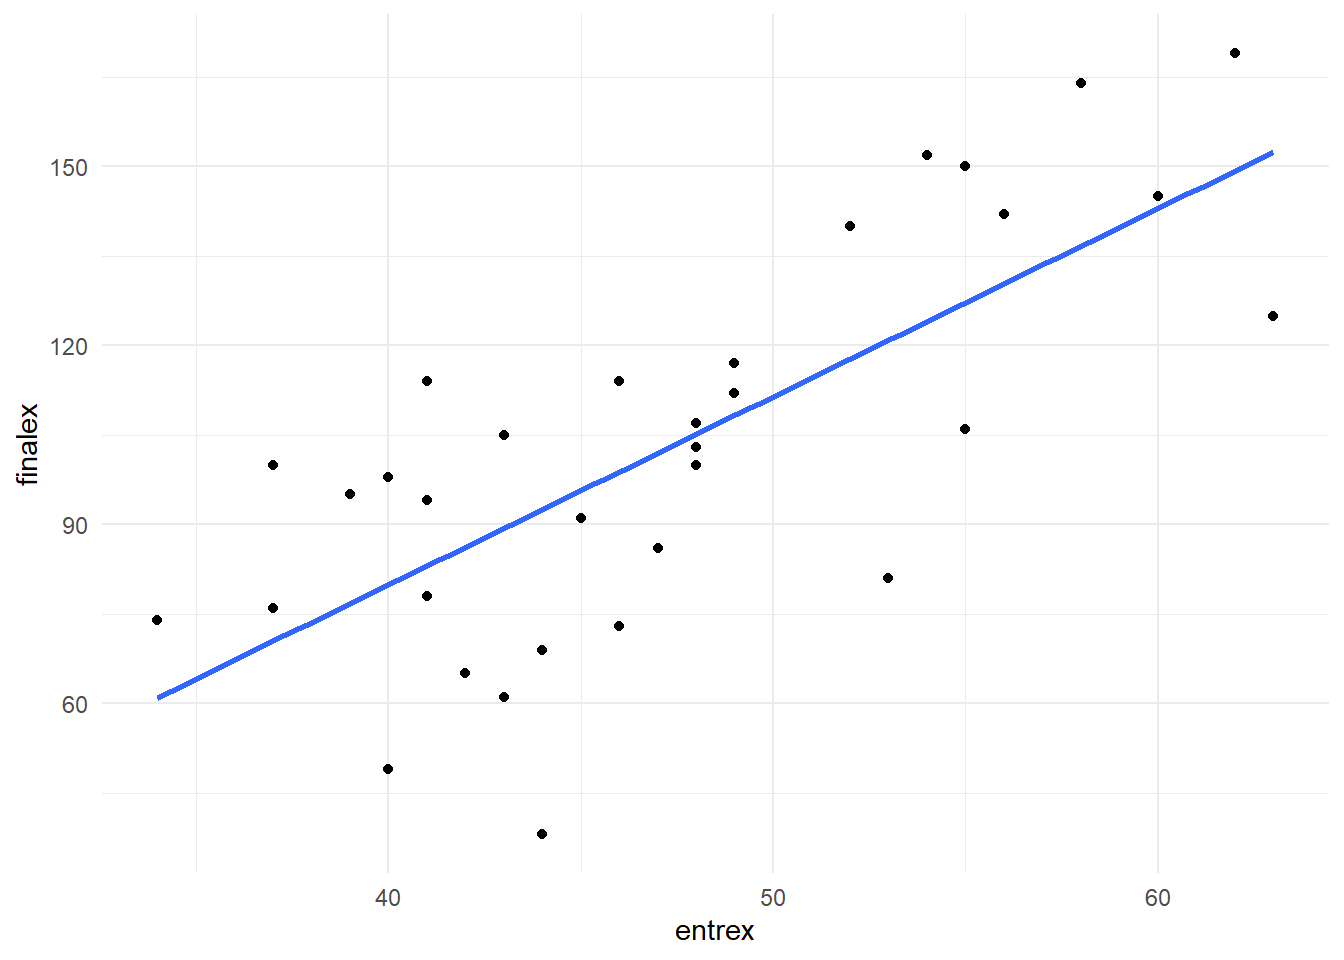
\includegraphics[width=1\linewidth]{02_multiple_regression_1_files/figure-latex/unnamed-chunk-3-1} 

}

\caption{TRUE}\label{fig:unnamed-chunk-3}
\end{figure}

There looks to be a positive association - students with higher entrance exam scores tend to have higher final exam scores. A good start!

To conduct the simple regression with \texttt{finalex} as the outcome variable, and \texttt{entrex} as the predictor variable, use \texttt{lm}:

\begin{Shaded}
\begin{Highlighting}[]
\NormalTok{m1 }\OtherTok{\textless{}{-}} \FunctionTok{lm}\NormalTok{(finalex }\SpecialCharTok{\textasciitilde{}}\NormalTok{ entrex, }\AttributeTok{data =}\NormalTok{ ExamData) }
\end{Highlighting}
\end{Shaded}

\textbf{Explanation}: \texttt{finalex\ \textasciitilde{}\ entrex} can be read as ``\texttt{finalex} is predicted by \texttt{entrex}''. The model is stored in \texttt{m1}.

View the intercept of the regression line and the coefficient for \texttt{entrex}:

\begin{Shaded}
\begin{Highlighting}[]
\NormalTok{m1}
\SpecialCharTok{\textgreater{}} 
\ErrorTok{\textgreater{}}\NormalTok{ Call}\SpecialCharTok{:}
\ErrorTok{\textgreater{}} \FunctionTok{lm}\NormalTok{(}\AttributeTok{formula =}\NormalTok{ finalex }\SpecialCharTok{\textasciitilde{}}\NormalTok{ entrex, }\AttributeTok{data =}\NormalTok{ ExamData)}
\SpecialCharTok{\textgreater{}} 
\ErrorTok{\textgreater{}}\NormalTok{ Coefficients}\SpecialCharTok{:}
\ErrorTok{\textgreater{}}\NormalTok{ (Intercept)       entrex  }
\SpecialCharTok{\textgreater{}}     \SpecialCharTok{{-}}\FloatTok{46.305}        \FloatTok{3.155}
\end{Highlighting}
\end{Shaded}

We can therefore write the regression equation:

\(Predicted\ final\ exam\ score = -46.305 + 3.155(entrance\ exam)\)

\hfill\break
\hfill\break
Use \texttt{summary(m1)} to display statistical analysis of the model:

\begin{Shaded}
\begin{Highlighting}[]
\FunctionTok{summary}\NormalTok{(m1)}
\SpecialCharTok{\textgreater{}} 
\ErrorTok{\textgreater{}}\NormalTok{ Call}\SpecialCharTok{:}
\ErrorTok{\textgreater{}} \FunctionTok{lm}\NormalTok{(}\AttributeTok{formula =}\NormalTok{ finalex }\SpecialCharTok{\textasciitilde{}}\NormalTok{ entrex, }\AttributeTok{data =}\NormalTok{ ExamData)}
\SpecialCharTok{\textgreater{}} 
\ErrorTok{\textgreater{}}\NormalTok{ Residuals}\SpecialCharTok{:}
\ErrorTok{\textgreater{}}\NormalTok{     Min      1Q  Median      3Q     Max }
\SpecialCharTok{\textgreater{}} \SpecialCharTok{{-}}\FloatTok{54.494} \SpecialCharTok{{-}}\FloatTok{21.185}   \FloatTok{3.733}  \FloatTok{18.124}  \FloatTok{30.969} 
\SpecialCharTok{\textgreater{}} 
\ErrorTok{\textgreater{}}\NormalTok{ Coefficients}\SpecialCharTok{:}
\ErrorTok{\textgreater{}}\NormalTok{             Estimate Std. Error t value }\FunctionTok{Pr}\NormalTok{(}\SpecialCharTok{\textgreater{}}\ErrorTok{|}\NormalTok{t}\SpecialCharTok{|}\NormalTok{)    }
\SpecialCharTok{\textgreater{}}\NormalTok{ (Intercept) }\SpecialCharTok{{-}}\FloatTok{46.3045}    \FloatTok{25.4773}  \SpecialCharTok{{-}}\FloatTok{1.817}   \FloatTok{0.0788}\NormalTok{ .  }
\SpecialCharTok{\textgreater{}}\NormalTok{ entrex        }\FloatTok{3.1545}     \FloatTok{0.5324}   \FloatTok{5.925} \FloatTok{1.52e{-}06} \SpecialCharTok{**}\ErrorTok{*}
\ErrorTok{\textgreater{}} \SpecialCharTok{{-}{-}{-}}
\ErrorTok{\textgreater{}}\NormalTok{ Signif. codes}\SpecialCharTok{:}  \DecValTok{0} \StringTok{\textquotesingle{}***\textquotesingle{}} \FloatTok{0.001} \StringTok{\textquotesingle{}**\textquotesingle{}} \FloatTok{0.01} \StringTok{\textquotesingle{}*\textquotesingle{}} \FloatTok{0.05} \StringTok{\textquotesingle{}.\textquotesingle{}} \FloatTok{0.1} \StringTok{\textquotesingle{} \textquotesingle{}} \DecValTok{1}
\SpecialCharTok{\textgreater{}} 
\ErrorTok{\textgreater{}}\NormalTok{ Residual standard error}\SpecialCharTok{:} \FloatTok{22.7}\NormalTok{ on }\DecValTok{31}\NormalTok{ degrees of freedom}
\SpecialCharTok{\textgreater{}}\NormalTok{ Multiple R}\SpecialCharTok{{-}}\NormalTok{squared}\SpecialCharTok{:}  \FloatTok{0.531}\NormalTok{,   Adjusted R}\SpecialCharTok{{-}}\NormalTok{squared}\SpecialCharTok{:}  \FloatTok{0.5159} 
\SpecialCharTok{\textgreater{}}\NormalTok{ F}\SpecialCharTok{{-}}\NormalTok{statistic}\SpecialCharTok{:}  \FloatTok{35.1}\NormalTok{ on }\DecValTok{1}\NormalTok{ and }\DecValTok{31}\NormalTok{ DF,  p}\SpecialCharTok{{-}}\NormalTok{value}\SpecialCharTok{:} \FloatTok{1.52e{-}06}
\end{Highlighting}
\end{Shaded}

\textbf{Explanation of the output}:

\hfill\break
\textbf{\texttt{Residuals:}} provides an indication of the discrepancy between the values of \texttt{finalex} predicted by the model (i.e., the regression equation) and the actual values of \texttt{finalex}. If the model does a good job in predicting \texttt{finalex}, the residuals should be relatively small.

\begin{itemize}
\tightlist
\item
  The difference between \texttt{Min} and \texttt{Max} gives us some idea of the range of error in the prediction of \texttt{finalex} scores. The difference in \texttt{3Q} and \texttt{1Q} is the interquartile range. The \texttt{median} of the residuals is 3.73.
\end{itemize}

\hfill\break
\textbf{\texttt{Coefficients:}} contains tests of statistical significance for each of the coefficients. The values in the column headed \texttt{Pr(\textgreater{}\textbar{}t\textbar{})} are the \emph{p}-values associated with the \emph{t}-values for the coefficients for each predictor. The \emph{t}-values test a null hypothesis that the coefficients are equal to zero. A \emph{p}-value less than .05 indicates that a predictor is statistically significant.

\begin{itemize}
\item
  The row for the \texttt{(intercept)} reports a \emph{t}-test for whether the value of the intercept differs from zero. We're not usually interested in this test (so don't report it).
\item
  The row for \texttt{entrex} tests whether the value of its coefficient (3.15) differs from zero. A coefficient of zero would be expected if the predictor explained no variance in the outcome variable. The coefficient for \texttt{entrex} (3.15) is clearly greater than zero. We can report this by saying that \texttt{extrex} is a statistically significant predictor of \texttt{finalex}, \emph{b} = 3.15, \emph{t}(31) = 5.92, \emph{p} \textless{} .001.
\end{itemize}

\hfill\break
\textbf{\texttt{Multiple\ R-squared:}} This is \(R^2\) - the \textbf{proportion of variance in \texttt{finalex} explained by \texttt{entrex}}. Here, \(R^2\) = 0.531. So approximately half of the variance in \texttt{finalex} is explained by \texttt{entrex}. It's usually referred to simply as ``R-squared'' or \(R^2\).

\begin{itemize}
\tightlist
\item
  \(R^2\) is often reported as a percentage. To get this, simply multiply the value by 100. i.e., 0.531 x 100 = 53.10\%.
\end{itemize}

\hfill\break
\textbf{\texttt{Adjusted\ R-squared:}} is an estimate of \(R^2\), but adjusted for the population. Despite the usefulness of this statistic, most studies still tend to report only the (unadjusted) \(R^2\) value. If reporting the \texttt{Adjusted\ R-squared} value, be sure to label it clearly as such. Here, Adjusted R-squared = 0.52.

\hfill\break
\textbf{\texttt{F-statistic:}} This compares the variance in \texttt{finalex} explained by the model with the variance that it does not explain (i.e., explained variance divided by unexplained variance). Higher values of \emph{F} indicate that the model explains greater variance in an outcome variable. If the \emph{p}-value associated with the \emph{F}-statistic is less than .05, we can say that the model significantly predicts the outcome variable.

Hence, we can say that a model consisting of \texttt{entrex} alone is a significant predictor of \texttt{finalex}, \emph{F}(1, 31) = 35.10, \emph{p} \textless{} .001. Higher \texttt{entrex} scores tend to be associated with higher \texttt{finalex} scores. If our model did not explain any variance in \texttt{finalex}, we wouldn't expect this to be statistically significant.

\begin{itemize}
\tightlist
\item
  In simple regression, the null hypothesis being tested on the \emph{F}-statistic is that the slope of the regression line in the population is equal to zero. This is actually equivalent to the \emph{t}-test on the \texttt{entrex} coefficient. So in simple regression, report the \emph{F}-statistic for the overall regression or the \emph{t}-test on the coefficient (not both). This equivalence between \emph{F} and \emph{t} does not hold true for multiple regression, as we shall see later.
\end{itemize}

\begin{exercise}

\textbf{Now you have a go}

Run another simple regression:

\begin{itemize}
\item
  set \texttt{finalex} as the outcome variable and \texttt{project} as the predictor variable
\item
  store the output in a variable with a different name (\texttt{m2})
\item
  then display the output of \texttt{m2} using \texttt{summary()}.
\end{itemize}

Try yourself first before clicking to show the code

\begin{Shaded}
\begin{Highlighting}[]
\NormalTok{m2 }\OtherTok{\textless{}{-}} \FunctionTok{lm}\NormalTok{(finalex }\SpecialCharTok{\textasciitilde{}}\NormalTok{ project, }\AttributeTok{data=}\NormalTok{ ExamData) }

\FunctionTok{summary}\NormalTok{(m2)}
\SpecialCharTok{\textgreater{}} 
\ErrorTok{\textgreater{}}\NormalTok{ Call}\SpecialCharTok{:}
\ErrorTok{\textgreater{}} \FunctionTok{lm}\NormalTok{(}\AttributeTok{formula =}\NormalTok{ finalex }\SpecialCharTok{\textasciitilde{}}\NormalTok{ project, }\AttributeTok{data =}\NormalTok{ ExamData)}
\SpecialCharTok{\textgreater{}} 
\ErrorTok{\textgreater{}}\NormalTok{ Residuals}\SpecialCharTok{:}
\ErrorTok{\textgreater{}}\NormalTok{     Min      1Q  Median      3Q     Max }
\SpecialCharTok{\textgreater{}} \SpecialCharTok{{-}}\FloatTok{64.015} \SpecialCharTok{{-}}\FloatTok{21.686}  \SpecialCharTok{{-}}\FloatTok{0.573}  \FloatTok{21.758}  \FloatTok{70.427} 
\SpecialCharTok{\textgreater{}} 
\ErrorTok{\textgreater{}}\NormalTok{ Coefficients}\SpecialCharTok{:}
\ErrorTok{\textgreater{}}\NormalTok{             Estimate Std. Error t value }\FunctionTok{Pr}\NormalTok{(}\SpecialCharTok{\textgreater{}}\ErrorTok{|}\NormalTok{t}\SpecialCharTok{|}\NormalTok{)  }
\SpecialCharTok{\textgreater{}}\NormalTok{ (Intercept)   }\FloatTok{4.6968}    \FloatTok{40.1677}   \FloatTok{0.117}   \FloatTok{0.9077}  
\SpecialCharTok{\textgreater{}}\NormalTok{ project       }\FloatTok{1.4442}     \FloatTok{0.5861}   \FloatTok{2.464}   \FloatTok{0.0195} \SpecialCharTok{*}
\ErrorTok{\textgreater{}} \SpecialCharTok{{-}{-}{-}}
\ErrorTok{\textgreater{}}\NormalTok{ Signif. codes}\SpecialCharTok{:}  \DecValTok{0} \StringTok{\textquotesingle{}***\textquotesingle{}} \FloatTok{0.001} \StringTok{\textquotesingle{}**\textquotesingle{}} \FloatTok{0.01} \StringTok{\textquotesingle{}*\textquotesingle{}} \FloatTok{0.05} \StringTok{\textquotesingle{}.\textquotesingle{}} \FloatTok{0.1} \StringTok{\textquotesingle{} \textquotesingle{}} \DecValTok{1}
\SpecialCharTok{\textgreater{}} 
\ErrorTok{\textgreater{}}\NormalTok{ Residual standard error}\SpecialCharTok{:} \FloatTok{30.32}\NormalTok{ on }\DecValTok{31}\NormalTok{ degrees of freedom}
\SpecialCharTok{\textgreater{}}\NormalTok{ Multiple R}\SpecialCharTok{{-}}\NormalTok{squared}\SpecialCharTok{:}  \FloatTok{0.1638}\NormalTok{,  Adjusted R}\SpecialCharTok{{-}}\NormalTok{squared}\SpecialCharTok{:}  \FloatTok{0.1368} 
\SpecialCharTok{\textgreater{}}\NormalTok{ F}\SpecialCharTok{{-}}\NormalTok{statistic}\SpecialCharTok{:} \FloatTok{6.072}\NormalTok{ on }\DecValTok{1}\NormalTok{ and }\DecValTok{31}\NormalTok{ DF,  p}\SpecialCharTok{{-}}\NormalTok{value}\SpecialCharTok{:} \FloatTok{0.01948}
\end{Highlighting}
\end{Shaded}

\hfill\break
Answer the following: (report statistics to 2 decimal places)

\begin{itemize}
\item
  What is the value of the coefficient for \texttt{project}?
\item
  What proportion of the variance in \texttt{finalex} is explained by \texttt{project}?: \(R^2\) = (or \%).
\item
  Write down the regression equation (on a bit of paper).
\end{itemize}

Show me

\begin{itemize}
\tightlist
\item
  \(Predicted\ final\ exam\ score = 4.70 + 1.44(project)\)
\end{itemize}

\begin{itemize}
\item
  Is \texttt{project} alone a statistically significant predictor of \texttt{finalex}, as indicated by the \emph{F}-statistic? noyes
\item
  Report the \emph{F}-ratio in APA style, that is, in the form

  \textbf{\emph{F}(df1, df2) = \emph{F}-statistic, \emph{p} = \emph{p}-value}:
\end{itemize}

Show me

\emph{F}(1, 31) = 6.07, \emph{p} = .02

\begin{itemize}
\tightlist
\item
  Individuals with lowerhigher project scores tended to have higher final exam scores.
\end{itemize}

\end{exercise}

\hypertarget{conceptualising-the-variance-explained-by-predictors}{%
\section{Conceptualising the variance explained by predictors}\label{conceptualising-the-variance-explained-by-predictors}}

Venn diagrams are useful for understanding the variance that predictors explain in the outcome variable. They are especially useful for understanding what's going on in multiple regression.

Suppose the rectangle below represents all of the \emph{variance} in \texttt{finalex} to be explained.

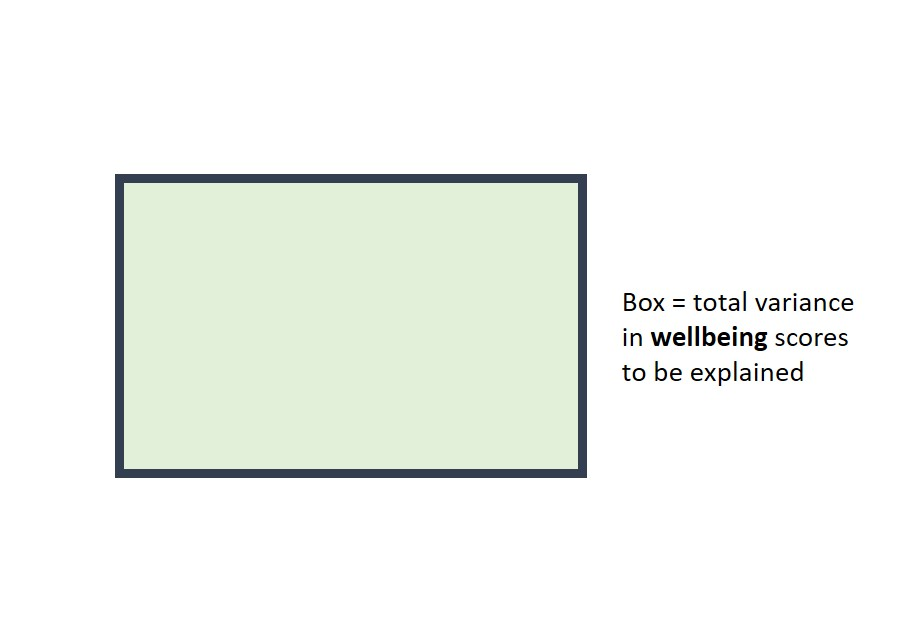
\includegraphics{images/Venn1.jpg}

The area of the circle below represents the variance in \texttt{finalex} explained by \texttt{entrex} in the first simple regression we did. If this diagram were drawn to scale (it's not), the area of the circle would be equal to the value of \(R^2\) (i.e., 53.1\% of the rectangle).

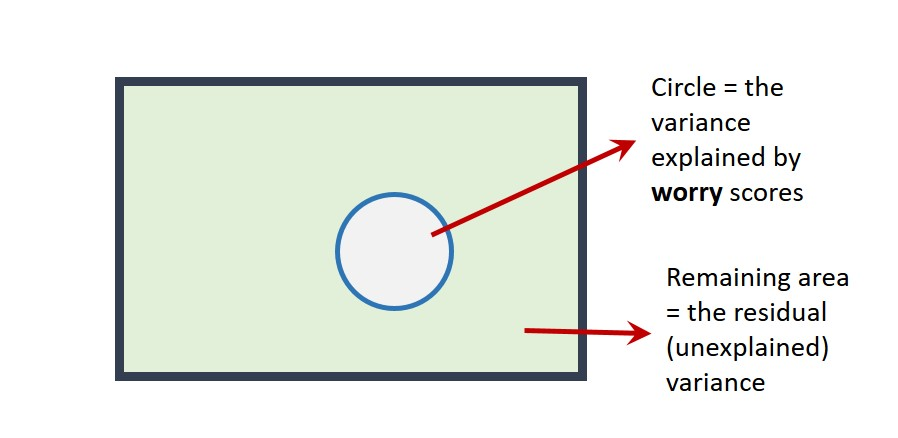
\includegraphics{images/Venn2.jpg}

The part of the rectangle not inside the circle represents the variance in \texttt{finalex} that is \emph{not} explained by the model (i.e., the unexplained or \emph{residual} variance).

To \emph{improve} the model, we can explore whether adding in other predictors to the model explains additional variance, thereby increasing the total \(R^2\) of the model.

You might think that we can simply add in variables (circles, above) to the model as we wish, until all the residual variance has been explained. This seems fine to do until we learn that if we were to add as many predictors to the model as there are rows in our data (33 individuals in our \texttt{ExamData}), then we'd perfectly predict the outcome variable, and have an \(R^2\) of 100\%! This would be true even if the predictors consisted of random values. Our model would clearly be meaningless though. We ideally want to explain the outcome variable with relatively few predictors.

\hypertarget{adding-predictor-variables-to-the-model}{%
\section{Adding predictor variables to the model}\label{adding-predictor-variables-to-the-model}}

An issue that can arise when adding variables to a model is that predictors are usually correlated to some extent. This can make interpretation of multiple regressions tricky. For example, a predictor that is statistically significant in a simple regression may become non-significant in a multiple regression. Let's see a demonstration of this!

We'll now add \texttt{project} to the model with \texttt{entrex}. First, check the correlation between predictors:

\begin{Shaded}
\begin{Highlighting}[]
\NormalTok{ExamData }\SpecialCharTok{\%\textgreater{}\%} 
  \FunctionTok{select}\NormalTok{(entrex,project) }\SpecialCharTok{\%\textgreater{}\%} 
  \FunctionTok{cor}\NormalTok{()}
\SpecialCharTok{\textgreater{}}\NormalTok{            entrex   project}
\SpecialCharTok{\textgreater{}}\NormalTok{ entrex  }\FloatTok{1.0000000} \FloatTok{0.2908253}
\SpecialCharTok{\textgreater{}}\NormalTok{ project }\FloatTok{0.2908253} \FloatTok{1.0000000}
\end{Highlighting}
\end{Shaded}

\begin{exercise}
The correlation between \texttt{entrex} and \texttt{project} is \emph{r} =

Our predictor variables are weakly correlated. We should keep this in mind going forward.
\end{exercise}

Now run a \emph{multiple regression} to predict \texttt{finalex} from both \texttt{entrex} and \texttt{project}. Again, use \texttt{lm} but use the \texttt{+} symbol to add predictors to the model:

\begin{Shaded}
\begin{Highlighting}[]
\NormalTok{m3 }\OtherTok{\textless{}{-}} \FunctionTok{lm}\NormalTok{(finalex }\SpecialCharTok{\textasciitilde{}}\NormalTok{ entrex }\SpecialCharTok{+}\NormalTok{ project, }\AttributeTok{data =}\NormalTok{ ExamData)}

\FunctionTok{summary}\NormalTok{(m3)}
\SpecialCharTok{\textgreater{}} 
\ErrorTok{\textgreater{}}\NormalTok{ Call}\SpecialCharTok{:}
\ErrorTok{\textgreater{}} \FunctionTok{lm}\NormalTok{(}\AttributeTok{formula =}\NormalTok{ finalex }\SpecialCharTok{\textasciitilde{}}\NormalTok{ entrex }\SpecialCharTok{+}\NormalTok{ project, }\AttributeTok{data =}\NormalTok{ ExamData)}
\SpecialCharTok{\textgreater{}} 
\ErrorTok{\textgreater{}}\NormalTok{ Residuals}\SpecialCharTok{:}
\ErrorTok{\textgreater{}}\NormalTok{     Min      1Q  Median      3Q     Max }
\SpecialCharTok{\textgreater{}} \SpecialCharTok{{-}}\FloatTok{41.880} \SpecialCharTok{{-}}\FloatTok{16.617}   \FloatTok{4.636}  \FloatTok{15.562}  \FloatTok{35.273} 
\SpecialCharTok{\textgreater{}} 
\ErrorTok{\textgreater{}}\NormalTok{ Coefficients}\SpecialCharTok{:}
\ErrorTok{\textgreater{}}\NormalTok{             Estimate Std. Error t value }\FunctionTok{Pr}\NormalTok{(}\SpecialCharTok{\textgreater{}}\ErrorTok{|}\NormalTok{t}\SpecialCharTok{|}\NormalTok{)    }
\SpecialCharTok{\textgreater{}}\NormalTok{ (Intercept) }\SpecialCharTok{{-}}\FloatTok{84.8289}    \FloatTok{33.6846}  \SpecialCharTok{{-}}\FloatTok{2.518}   \FloatTok{0.0174} \SpecialCharTok{*}  
\ErrorTok{\textgreater{}}\NormalTok{ entrex        }\FloatTok{2.8894}     \FloatTok{0.5406}   \FloatTok{5.344} \FloatTok{8.81e{-}06} \SpecialCharTok{**}\ErrorTok{*}
\ErrorTok{\textgreater{}}\NormalTok{ project       }\FloatTok{0.7515}     \FloatTok{0.4457}   \FloatTok{1.686}   \FloatTok{0.1021}    
\SpecialCharTok{\textgreater{}} \SpecialCharTok{{-}{-}{-}}
\ErrorTok{\textgreater{}}\NormalTok{ Signif. codes}\SpecialCharTok{:}  \DecValTok{0} \StringTok{\textquotesingle{}***\textquotesingle{}} \FloatTok{0.001} \StringTok{\textquotesingle{}**\textquotesingle{}} \FloatTok{0.01} \StringTok{\textquotesingle{}*\textquotesingle{}} \FloatTok{0.05} \StringTok{\textquotesingle{}.\textquotesingle{}} \FloatTok{0.1} \StringTok{\textquotesingle{} \textquotesingle{}} \DecValTok{1}
\SpecialCharTok{\textgreater{}} 
\ErrorTok{\textgreater{}}\NormalTok{ Residual standard error}\SpecialCharTok{:} \FloatTok{22.06}\NormalTok{ on }\DecValTok{30}\NormalTok{ degrees of freedom}
\SpecialCharTok{\textgreater{}}\NormalTok{ Multiple R}\SpecialCharTok{{-}}\NormalTok{squared}\SpecialCharTok{:}  \FloatTok{0.5716}\NormalTok{,  Adjusted R}\SpecialCharTok{{-}}\NormalTok{squared}\SpecialCharTok{:}  \FloatTok{0.5431} 
\SpecialCharTok{\textgreater{}}\NormalTok{ F}\SpecialCharTok{{-}}\NormalTok{statistic}\SpecialCharTok{:} \FloatTok{20.02}\NormalTok{ on }\DecValTok{2}\NormalTok{ and }\DecValTok{30}\NormalTok{ DF,  p}\SpecialCharTok{{-}}\NormalTok{value}\SpecialCharTok{:} \FloatTok{3e{-}06}
\end{Highlighting}
\end{Shaded}

\begin{exercise}

In this model with \texttt{entrex} and \texttt{project}as predictors:

What is the value of \(R^2\) (as a percentage): \%

By how much has \(R^2\) \emph{increased} in this model, relative to the model with \texttt{entrex} alone (where \(R^2\) was 53.10\%)? (as a percentage) (you will need to calculate this) \%

Is the overall regression model predicting \texttt{finalex} on the basis of \texttt{entrex} and \texttt{project} statistically significant? yesno

\begin{itemize}
\item
  Is \texttt{entrex} a statistically significant predictor of \texttt{finalex}? yesno
\item
  We can report this in the following way: the \emph{t}-test on the coefficient for \texttt{entrex} is statistically significant, \emph{b} = 2.89, \emph{t}(30) = 5.34, \emph{p} \textless{} .001.
\item
  Is \texttt{project} a statistically significant predictor of \texttt{finalex} in this model? yesno
\item
  What is the value of the coefficient for \texttt{project}? \emph{b} =
\item
  Report the \emph{t}-statistic in APA style:
\end{itemize}

Show me

Project mark was not a statistically significant predictor of final examination in this model, \emph{b} = 0.75, \emph{t}(30) = 1.69, \emph{p} = .10

\end{exercise}

Looking across the analyses we've performed, we can see that \texttt{project} is a (weak) but statistically significant predictor of \texttt{finalex} in a simple regression. However, when it is included in a model that also includes \texttt{entrex} it is not a significant predictor! What's going on?

\begin{itemize}
\item
  The model containing only \texttt{project} explains 16.38\% of the variability in \texttt{finalex}.
\item
  The model containing only \texttt{entrex} explains 53.10\% of the variability in \texttt{finalex}.
\item
  However, a model containing \emph{both} \texttt{project} and \texttt{entrex} only explains 57.16\% of the variability in \texttt{finalex}, not 16.38 + 53.10 = 69.48\%, as we might expect.
\end{itemize}

This is because the predictors are \emph{correlated} (\emph{r} = .29) and so the variance they explain in \texttt{finalex} is \emph{shared}.

\hfill\break
We could represent this on a Venn diagram as follows:

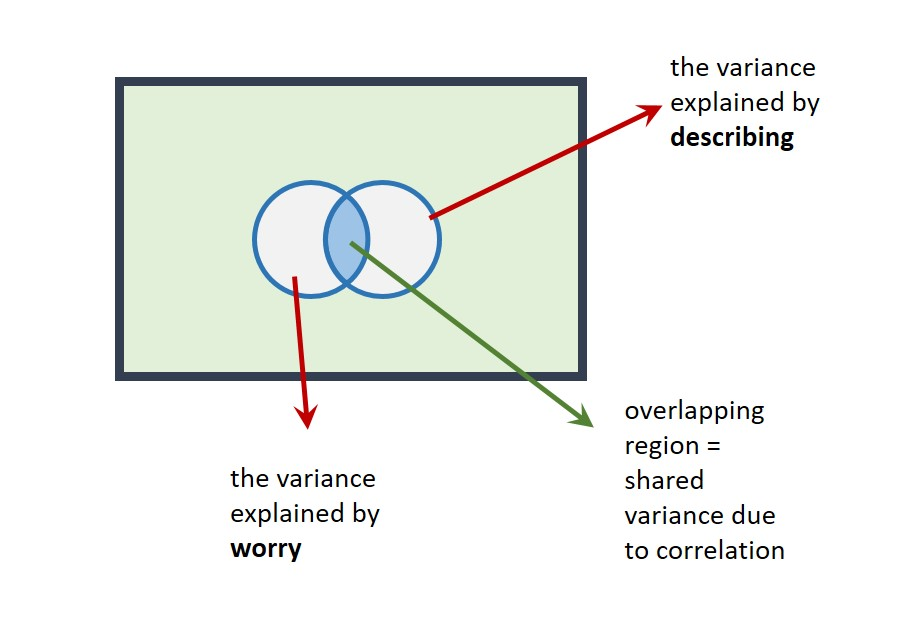
\includegraphics{images/Venn3.jpg}

The correlation is represented as an overlap in the circles. Their total area (57.16\%) is therefore \emph{less} than the area they'd explain if there were no overlap (69.48\%) (i.e., if there was no correlation).

\textbf{This demonstrates an important point}: The \emph{t}-tests on the coefficients in a multiple regression assess the \textbf{unique} contribution of each predictor in the model. That is, they test the variance a predictor explains in an outcome variable, \textbf{after} the variance explained by the other predictors has been taken into account. This is why \texttt{project} is not statistically significant in the multiple regression model -- it only explains a small amount of variance once \texttt{entrex} has been taken into account.

It is possible to think of the \emph{F}-statistic and \emph{t}-value in multiple regression in terms of the Venn diagram:

\begin{itemize}
\item
  The \textbf{\emph{F}-statistic} compares the explained variance with the unexplained variance. The explained variance is represented by the \textbf{\emph{outline}} of the two circles in the Venn diagram above. The unexplained variance is the remaining blue area of the rectangle.
\item
  The \textbf{\emph{t}-value} compares the unique variance a predictor explains with the remaining unexplained variance. For example, for \texttt{project} in the Venn diagram above, this would be the area in the orange \textbf{\emph{crescent}}, relative to the remaining blue area in the rectangle.
\end{itemize}

\hypertarget{multicollinearity}{%
\section{Multicollinearity}\label{multicollinearity}}

If the correlation between predictors is very high (greater than \emph{r} = 0.9), this is known as \textbf{multicollinearity}. On a Venn diagram, the circles representing the predictors would almost completely overlap. Multicollinearity can be a problem in multiple regression. Predictors may explain a large amount of variance in the outcome variable, but their `unique' contribution in a multiple regression may be small. A situation can arise where \emph{neither} predictor may be statistically significant even though the overall regression is significant!

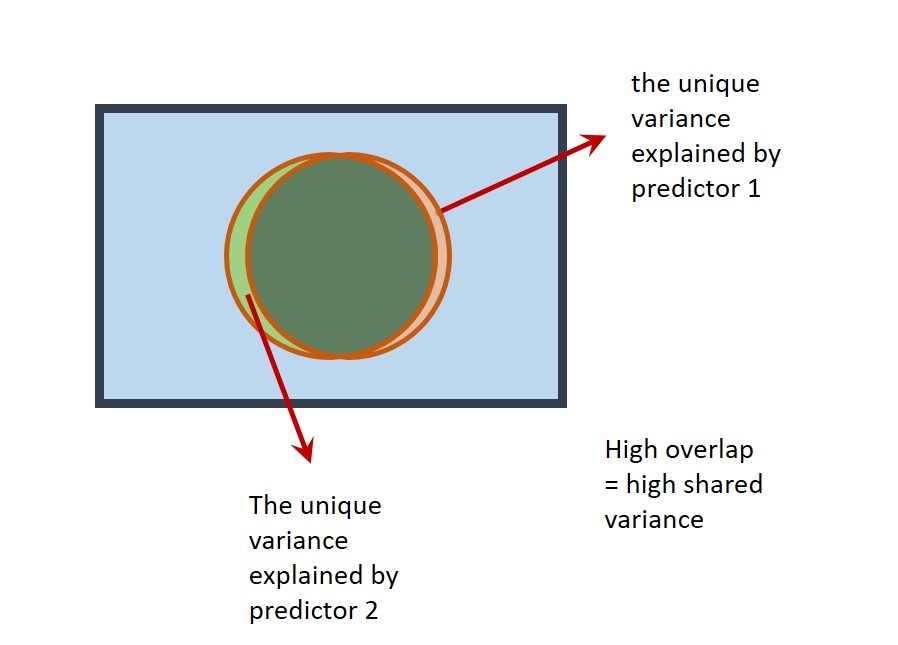
\includegraphics{images/Venn_multi.jpg}

An example of multicollinearity in the \texttt{ExamData} dataset can be seen with the variables \texttt{project} and \texttt{proposal}.

\begin{exercise}

Obtain the correlation between \texttt{project} and \texttt{proposal}:

Show me

\begin{Shaded}
\begin{Highlighting}[]
\NormalTok{ExamData }\SpecialCharTok{\%\textgreater{}\%} 
  \FunctionTok{select}\NormalTok{(project, proposal) }\SpecialCharTok{\%\textgreater{}\%} 
  \FunctionTok{cor}\NormalTok{()}
\SpecialCharTok{\textgreater{}}\NormalTok{            project  proposal}
\SpecialCharTok{\textgreater{}}\NormalTok{ project  }\FloatTok{1.0000000} \FloatTok{0.9371487}
\SpecialCharTok{\textgreater{}}\NormalTok{ proposal }\FloatTok{0.9371487} \FloatTok{1.0000000}
\end{Highlighting}
\end{Shaded}

The correlation between \texttt{project} and \texttt{proposal} is \emph{r} = .

To see the effects of multicollinearity, conduct a regression with \texttt{finalex} as the outcome variable and \texttt{project} and \texttt{proposal} as the predictor variables.

Show me

\begin{Shaded}
\begin{Highlighting}[]
\NormalTok{multi1 }\OtherTok{\textless{}{-}} \FunctionTok{lm}\NormalTok{(finalex }\SpecialCharTok{\textasciitilde{}}\NormalTok{ project }\SpecialCharTok{+}\NormalTok{ proposal, }\AttributeTok{data =}\NormalTok{ ExamData)}

\FunctionTok{summary}\NormalTok{(multi1)}
\SpecialCharTok{\textgreater{}} 
\ErrorTok{\textgreater{}}\NormalTok{ Call}\SpecialCharTok{:}
\ErrorTok{\textgreater{}} \FunctionTok{lm}\NormalTok{(}\AttributeTok{formula =}\NormalTok{ finalex }\SpecialCharTok{\textasciitilde{}}\NormalTok{ project }\SpecialCharTok{+}\NormalTok{ proposal, }\AttributeTok{data =}\NormalTok{ ExamData)}
\SpecialCharTok{\textgreater{}} 
\ErrorTok{\textgreater{}}\NormalTok{ Residuals}\SpecialCharTok{:}
\ErrorTok{\textgreater{}}\NormalTok{     Min      1Q  Median      3Q     Max }
\SpecialCharTok{\textgreater{}} \SpecialCharTok{{-}}\FloatTok{64.287} \SpecialCharTok{{-}}\FloatTok{22.590}  \SpecialCharTok{{-}}\FloatTok{0.346}  \FloatTok{22.395}  \FloatTok{70.289} 
\SpecialCharTok{\textgreater{}} 
\ErrorTok{\textgreater{}}\NormalTok{ Coefficients}\SpecialCharTok{:}
\ErrorTok{\textgreater{}}\NormalTok{             Estimate Std. Error t value }\FunctionTok{Pr}\NormalTok{(}\SpecialCharTok{\textgreater{}}\ErrorTok{|}\NormalTok{t}\SpecialCharTok{|}\NormalTok{)}
\SpecialCharTok{\textgreater{}}\NormalTok{ (Intercept)   }\FloatTok{4.8784}    \FloatTok{40.8601}   \FloatTok{0.119}    \FloatTok{0.906}
\SpecialCharTok{\textgreater{}}\NormalTok{ project       }\FloatTok{1.2751}     \FloatTok{1.7072}   \FloatTok{0.747}    \FloatTok{0.461}
\SpecialCharTok{\textgreater{}}\NormalTok{ proposal      }\FloatTok{0.1826}     \FloatTok{1.7263}   \FloatTok{0.106}    \FloatTok{0.916}
\SpecialCharTok{\textgreater{}} 
\ErrorTok{\textgreater{}}\NormalTok{ Residual standard error}\SpecialCharTok{:} \FloatTok{30.81}\NormalTok{ on }\DecValTok{30}\NormalTok{ degrees of freedom}
\SpecialCharTok{\textgreater{}}\NormalTok{ Multiple R}\SpecialCharTok{{-}}\NormalTok{squared}\SpecialCharTok{:}  \FloatTok{0.1641}\NormalTok{,  Adjusted R}\SpecialCharTok{{-}}\NormalTok{squared}\SpecialCharTok{:}  \FloatTok{0.1084} 
\SpecialCharTok{\textgreater{}}\NormalTok{ F}\SpecialCharTok{{-}}\NormalTok{statistic}\SpecialCharTok{:} \FloatTok{2.945}\NormalTok{ on }\DecValTok{2}\NormalTok{ and }\DecValTok{30}\NormalTok{ DF,  p}\SpecialCharTok{{-}}\NormalTok{value}\SpecialCharTok{:} \FloatTok{0.06797}
\end{Highlighting}
\end{Shaded}

\begin{itemize}
\item
  How much variance in \texttt{finalex} is explained by the model: \(R^2\) = \%.
\item
  Is the overall regression statistically significant? yesno
\item
  Is the coefficient for \texttt{project} statistically significant? yesno
\item
  Is the coefficient for \texttt{proposal} statistically significant? yesno
\end{itemize}

\end{exercise}

\begin{exercise}

Now run two simple regressions to determine whether \texttt{project} and \texttt{proposal} explain variance in \texttt{finalex} and are statistically significant predictors when in models on their own.

Show me

\begin{Shaded}
\begin{Highlighting}[]
\NormalTok{multi2 }\OtherTok{\textless{}{-}} \FunctionTok{lm}\NormalTok{(finalex }\SpecialCharTok{\textasciitilde{}}\NormalTok{ project, }\AttributeTok{data =}\NormalTok{ ExamData)}
\FunctionTok{summary}\NormalTok{(multi2)}

\NormalTok{multi3 }\OtherTok{\textless{}{-}} \FunctionTok{lm}\NormalTok{(finalex }\SpecialCharTok{\textasciitilde{}}\NormalTok{ proposal, }\AttributeTok{data =}\NormalTok{ ExamData)}
\FunctionTok{summary}\NormalTok{(multi3)}
\SpecialCharTok{\textgreater{}} 
\ErrorTok{\textgreater{}}\NormalTok{ Call}\SpecialCharTok{:}
\ErrorTok{\textgreater{}} \FunctionTok{lm}\NormalTok{(}\AttributeTok{formula =}\NormalTok{ finalex }\SpecialCharTok{\textasciitilde{}}\NormalTok{ project, }\AttributeTok{data =}\NormalTok{ ExamData)}
\SpecialCharTok{\textgreater{}} 
\ErrorTok{\textgreater{}}\NormalTok{ Residuals}\SpecialCharTok{:}
\ErrorTok{\textgreater{}}\NormalTok{     Min      1Q  Median      3Q     Max }
\SpecialCharTok{\textgreater{}} \SpecialCharTok{{-}}\FloatTok{64.015} \SpecialCharTok{{-}}\FloatTok{21.686}  \SpecialCharTok{{-}}\FloatTok{0.573}  \FloatTok{21.758}  \FloatTok{70.427} 
\SpecialCharTok{\textgreater{}} 
\ErrorTok{\textgreater{}}\NormalTok{ Coefficients}\SpecialCharTok{:}
\ErrorTok{\textgreater{}}\NormalTok{             Estimate Std. Error t value }\FunctionTok{Pr}\NormalTok{(}\SpecialCharTok{\textgreater{}}\ErrorTok{|}\NormalTok{t}\SpecialCharTok{|}\NormalTok{)  }
\SpecialCharTok{\textgreater{}}\NormalTok{ (Intercept)   }\FloatTok{4.6968}    \FloatTok{40.1677}   \FloatTok{0.117}   \FloatTok{0.9077}  
\SpecialCharTok{\textgreater{}}\NormalTok{ project       }\FloatTok{1.4442}     \FloatTok{0.5861}   \FloatTok{2.464}   \FloatTok{0.0195} \SpecialCharTok{*}
\ErrorTok{\textgreater{}} \SpecialCharTok{{-}{-}{-}}
\ErrorTok{\textgreater{}}\NormalTok{ Signif. codes}\SpecialCharTok{:}  \DecValTok{0} \StringTok{\textquotesingle{}***\textquotesingle{}} \FloatTok{0.001} \StringTok{\textquotesingle{}**\textquotesingle{}} \FloatTok{0.01} \StringTok{\textquotesingle{}*\textquotesingle{}} \FloatTok{0.05} \StringTok{\textquotesingle{}.\textquotesingle{}} \FloatTok{0.1} \StringTok{\textquotesingle{} \textquotesingle{}} \DecValTok{1}
\SpecialCharTok{\textgreater{}} 
\ErrorTok{\textgreater{}}\NormalTok{ Residual standard error}\SpecialCharTok{:} \FloatTok{30.32}\NormalTok{ on }\DecValTok{31}\NormalTok{ degrees of freedom}
\SpecialCharTok{\textgreater{}}\NormalTok{ Multiple R}\SpecialCharTok{{-}}\NormalTok{squared}\SpecialCharTok{:}  \FloatTok{0.1638}\NormalTok{,  Adjusted R}\SpecialCharTok{{-}}\NormalTok{squared}\SpecialCharTok{:}  \FloatTok{0.1368} 
\SpecialCharTok{\textgreater{}}\NormalTok{ F}\SpecialCharTok{{-}}\NormalTok{statistic}\SpecialCharTok{:} \FloatTok{6.072}\NormalTok{ on }\DecValTok{1}\NormalTok{ and }\DecValTok{31}\NormalTok{ DF,  p}\SpecialCharTok{{-}}\NormalTok{value}\SpecialCharTok{:} \FloatTok{0.01948}
\SpecialCharTok{\textgreater{}} 
\ErrorTok{\textgreater{}} 
\ErrorTok{\textgreater{}}\NormalTok{ Call}\SpecialCharTok{:}
\ErrorTok{\textgreater{}} \FunctionTok{lm}\NormalTok{(}\AttributeTok{formula =}\NormalTok{ finalex }\SpecialCharTok{\textasciitilde{}}\NormalTok{ proposal, }\AttributeTok{data =}\NormalTok{ ExamData)}
\SpecialCharTok{\textgreater{}} 
\ErrorTok{\textgreater{}}\NormalTok{ Residuals}\SpecialCharTok{:}
\ErrorTok{\textgreater{}}\NormalTok{     Min      1Q  Median      3Q     Max }
\SpecialCharTok{\textgreater{}} \SpecialCharTok{{-}}\FloatTok{64.987} \SpecialCharTok{{-}}\FloatTok{22.987}  \SpecialCharTok{{-}}\FloatTok{1.378}  \FloatTok{24.059}  \FloatTok{68.921} 
\SpecialCharTok{\textgreater{}} 
\ErrorTok{\textgreater{}}\NormalTok{ Coefficients}\SpecialCharTok{:}
\ErrorTok{\textgreater{}}\NormalTok{             Estimate Std. Error t value }\FunctionTok{Pr}\NormalTok{(}\SpecialCharTok{\textgreater{}}\ErrorTok{|}\NormalTok{t}\SpecialCharTok{|}\NormalTok{)  }
\SpecialCharTok{\textgreater{}}\NormalTok{ (Intercept)   }\FloatTok{16.628}     \FloatTok{37.441}   \FloatTok{0.444}   \FloatTok{0.6601}  
\SpecialCharTok{\textgreater{}}\NormalTok{ proposal       }\FloatTok{1.391}      \FloatTok{0.598}   \FloatTok{2.326}   \FloatTok{0.0267} \SpecialCharTok{*}
\ErrorTok{\textgreater{}} \SpecialCharTok{{-}{-}{-}}
\ErrorTok{\textgreater{}}\NormalTok{ Signif. codes}\SpecialCharTok{:}  \DecValTok{0} \StringTok{\textquotesingle{}***\textquotesingle{}} \FloatTok{0.001} \StringTok{\textquotesingle{}**\textquotesingle{}} \FloatTok{0.01} \StringTok{\textquotesingle{}*\textquotesingle{}} \FloatTok{0.05} \StringTok{\textquotesingle{}.\textquotesingle{}} \FloatTok{0.1} \StringTok{\textquotesingle{} \textquotesingle{}} \DecValTok{1}
\SpecialCharTok{\textgreater{}} 
\ErrorTok{\textgreater{}}\NormalTok{ Residual standard error}\SpecialCharTok{:} \FloatTok{30.59}\NormalTok{ on }\DecValTok{31}\NormalTok{ degrees of freedom}
\SpecialCharTok{\textgreater{}}\NormalTok{ Multiple R}\SpecialCharTok{{-}}\NormalTok{squared}\SpecialCharTok{:}  \FloatTok{0.1486}\NormalTok{,  Adjusted R}\SpecialCharTok{{-}}\NormalTok{squared}\SpecialCharTok{:}  \FloatTok{0.1211} 
\SpecialCharTok{\textgreater{}}\NormalTok{ F}\SpecialCharTok{{-}}\NormalTok{statistic}\SpecialCharTok{:} \FloatTok{5.409}\NormalTok{ on }\DecValTok{1}\NormalTok{ and }\DecValTok{31}\NormalTok{ DF,  p}\SpecialCharTok{{-}}\NormalTok{value}\SpecialCharTok{:} \FloatTok{0.02675}
\end{Highlighting}
\end{Shaded}

\begin{itemize}
\item
  In a simple regression with \texttt{finalex} as the outcome variable, and \texttt{project} as the predictor variable, \(R^2\) = \%.
\item
  Is the overall regression statistically significant? yesno
\item
  In a simple regression with \texttt{finalex} as the outcome variable, and \texttt{proposal} as the predictor variable, \(R^2\) = \%.
\item
  Is the overall regression statistically significant? yesno
\item
  Try to explain what's going on here in your own words. Click below or ask if you get stuck.
\end{itemize}

Explain

\emph{Interpretation}

\begin{itemize}
\item
  Because \texttt{proposal} and \texttt{project} are highly correlated (\emph{r} = 0.94), this gives rise to the situation where the simple regressions indicate that they explain variance in \texttt{finalex}, but when both are included as predictors in a multiple regression, it appears as if neither are significant predictors of \texttt{finalex} !
\item
  If this were a real scenario, we'd consider dropping \texttt{project} or \texttt{proposal} from the model. Because the correlation is so high, having one predictor is as good as having the other (more or less).
\item
  It seems intuitive that a person's final project mark would be highly correlated with their proposal mark.
\item
  The take-home message here is to check for high correlations between your predictor variables before including them in a multiple regression.
\end{itemize}

\end{exercise}

\hypertarget{final-exercise}{%
\section{Final exercise}\label{final-exercise}}

\begin{exercise}

As a final exercise, run a multiple regression to predict \texttt{finalex} from \textbf{three} predictors: \texttt{entrex}, \texttt{project}, and \texttt{iq}.

Show me how

\begin{Shaded}
\begin{Highlighting}[]
\NormalTok{multi4 }\OtherTok{\textless{}{-}} \FunctionTok{lm}\NormalTok{(finalex }\SpecialCharTok{\textasciitilde{}}\NormalTok{ entrex }\SpecialCharTok{+}\NormalTok{ project }\SpecialCharTok{+}\NormalTok{ iq, }\AttributeTok{data =}\NormalTok{ ExamData)}

\FunctionTok{summary}\NormalTok{(multi4)}
\SpecialCharTok{\textgreater{}} 
\ErrorTok{\textgreater{}}\NormalTok{ Call}\SpecialCharTok{:}
\ErrorTok{\textgreater{}} \FunctionTok{lm}\NormalTok{(}\AttributeTok{formula =}\NormalTok{ finalex }\SpecialCharTok{\textasciitilde{}}\NormalTok{ entrex }\SpecialCharTok{+}\NormalTok{ project }\SpecialCharTok{+}\NormalTok{ iq, }\AttributeTok{data =}\NormalTok{ ExamData)}
\SpecialCharTok{\textgreater{}} 
\ErrorTok{\textgreater{}}\NormalTok{ Residuals}\SpecialCharTok{:}
\ErrorTok{\textgreater{}}\NormalTok{     Min      1Q  Median      3Q     Max }
\SpecialCharTok{\textgreater{}} \SpecialCharTok{{-}}\FloatTok{40.444} \SpecialCharTok{{-}}\FloatTok{16.174}   \FloatTok{5.509}  \FloatTok{14.312}  \FloatTok{33.338} 
\SpecialCharTok{\textgreater{}} 
\ErrorTok{\textgreater{}}\NormalTok{ Coefficients}\SpecialCharTok{:}
\ErrorTok{\textgreater{}}\NormalTok{              Estimate Std. Error t value }\FunctionTok{Pr}\NormalTok{(}\SpecialCharTok{\textgreater{}}\ErrorTok{|}\NormalTok{t}\SpecialCharTok{|}\NormalTok{)    }
\SpecialCharTok{\textgreater{}}\NormalTok{ (Intercept) }\SpecialCharTok{{-}}\FloatTok{130.3803}    \FloatTok{54.7288}  \SpecialCharTok{{-}}\FloatTok{2.382} \FloatTok{0.023981} \SpecialCharTok{*}  
\ErrorTok{\textgreater{}}\NormalTok{ entrex         }\FloatTok{2.6180}     \FloatTok{0.5978}   \FloatTok{4.379} \FloatTok{0.000142} \SpecialCharTok{**}\ErrorTok{*}
\ErrorTok{\textgreater{}}\NormalTok{ project        }\FloatTok{0.6874}     \FloatTok{0.4490}   \FloatTok{1.531} \FloatTok{0.136620}    
\SpecialCharTok{\textgreater{}}\NormalTok{ iq             }\FloatTok{0.4862}     \FloatTok{0.4610}   \FloatTok{1.055} \FloatTok{0.300214}    
\SpecialCharTok{\textgreater{}} \SpecialCharTok{{-}{-}{-}}
\ErrorTok{\textgreater{}}\NormalTok{ Signif. codes}\SpecialCharTok{:}  \DecValTok{0} \StringTok{\textquotesingle{}***\textquotesingle{}} \FloatTok{0.001} \StringTok{\textquotesingle{}**\textquotesingle{}} \FloatTok{0.01} \StringTok{\textquotesingle{}*\textquotesingle{}} \FloatTok{0.05} \StringTok{\textquotesingle{}.\textquotesingle{}} \FloatTok{0.1} \StringTok{\textquotesingle{} \textquotesingle{}} \DecValTok{1}
\SpecialCharTok{\textgreater{}} 
\ErrorTok{\textgreater{}}\NormalTok{ Residual standard error}\SpecialCharTok{:} \FloatTok{22.02}\NormalTok{ on }\DecValTok{29}\NormalTok{ degrees of freedom}
\SpecialCharTok{\textgreater{}}\NormalTok{ Multiple R}\SpecialCharTok{{-}}\NormalTok{squared}\SpecialCharTok{:}  \FloatTok{0.5875}\NormalTok{,  Adjusted R}\SpecialCharTok{{-}}\NormalTok{squared}\SpecialCharTok{:}  \FloatTok{0.5448} 
\SpecialCharTok{\textgreater{}}\NormalTok{ F}\SpecialCharTok{{-}}\NormalTok{statistic}\SpecialCharTok{:} \FloatTok{13.77}\NormalTok{ on }\DecValTok{3}\NormalTok{ and }\DecValTok{29}\NormalTok{ DF,  p}\SpecialCharTok{{-}}\NormalTok{value}\SpecialCharTok{:} \FloatTok{9.168e{-}06}
\end{Highlighting}
\end{Shaded}

Which variables are statistically significant predictors of \texttt{finalex}?

\begin{itemize}
\item
  \texttt{entrex} yesno
\item
  \texttt{project} yesno
\item
  \texttt{iq} yesno
\end{itemize}

On the basis of all the models conducted so far (with \texttt{entrex}, \texttt{project}, and \texttt{iq}), which model would you choose to best predict \texttt{finalex}?

Tell me which model seems best

The model containing \texttt{entrex} alone, as this seems to provide the simplest and most effective model of the \texttt{finalex}.

A general goal of regression is to identify the fewest predictor variables necessary to predict an outcome variable, where each predictor variable predicts a substantial and independent segment of the variability in the outcome variable.

\end{exercise}

\hypertarget{summary-of-key-points}{%
\section{Summary of key points}\label{summary-of-key-points}}

\begin{itemize}
\item
  Predictors can be added to a model in \texttt{lm} using the \texttt{+} symbol
\item
  e.g., \texttt{lm(finalex\ \textasciitilde{}\ entrex\ +\ project\ +\ iq)}
\item
  Predictor variables are often correlated to some extent. This can affect the interpretation of individual predictor variables. Venn diagrams help to understand the results.
\item
  The \textbf{\emph{F}-statistic} tells us whether the model \emph{as a whole} significantly predicts the outcome variable.
\item
  The \textbf{\emph{t}-values} tell us whether individual predictors in the model are statistically significant.
\item
  In multiple regression, it's important to understand that the statistical significance of individual predictors only holds \textbf{after taking into account the other predictors in the model}.
\item
  \textbf{Multicollinearity} exists when predictors are very highly correlated (\emph{r} above 0.9) and should be avoided.
\end{itemize}

\hypertarget{anova-2x2-between-subjects}{%
\chapter{ANOVA: 2x2 Between-subjects}\label{anova-2x2-between-subjects}}

\hypertarget{multiple-regression-one-continuous-one-categorical}{%
\chapter{Multiple regression: one continuous, one categorical}\label{multiple-regression-one-continuous-one-categorical}}

\hypertarget{multiple3}{%
\chapter{Multiple regression: evaluating and comparing models}\label{multiple3}}

\emph{January 2022}

\hypertarget{in-brief-1}{%
\subsection{In brief}\label{in-brief-1}}

\begin{quote}
In this session we discuss model selection in the context of ANOVA and the use
of Bayes Factors to choose between theoretically interesting models.
\end{quote}

\hypertarget{using-anova-and-bayes-factors-to-compare-models}{%
\section{Using ANOVA and Bayes Factors to compare models}\label{using-anova-and-bayes-factors-to-compare-models}}

\begin{itemize}
\tightlist
\item
  \href{slides/PSYC753_Chris2.pptx}{\textbf{Slides for the session}}
\item
  \href{slides/PSYC753_Chris2_Rmd.pptx}{\textbf{Using Rmd files}}
\end{itemize}

\hfill\break

\hypertarget{overview-2}{%
\subsection{Overview}\label{overview-2}}

In the previous session, we saw that we can construct a linear model to predict an outcome variable (e.g., \emph{final exam score} from \emph{entrance exam score}). We also investigated how we can \emph{improve} a model by adding several continuous predictors to it.

\hfill\break
How do we know if one model is \emph{better} or should be \emph{preferred} over another model? We touched on a common sense approach in the last session - we ideally want models that explain the variance in an outcome variable but each predictor in the model should make a sizable and relatively independent contribution to the model.

\hfill\break

Today we will cover a more formal approach to model comparison using:

\begin{itemize}
\item
  \textbf{ANOVA (Analysis of Variance)} and
\item
  \textbf{Bayes Factors}
\end{itemize}

\hfill\break

It's important that you are comfortable with the material from the first \href{building-models-1.html}{Building Models 1 session} before proceeding today.

\hypertarget{comparing-models-using-anova}{%
\section{Comparing models using ANOVA}\label{comparing-models-using-anova}}

We can use ANOVA to determine whether the addition of variables into a model leads to a statistically significant improvement in the variance it explains \emph{overall}. We may want to do this, for example, when building on existing theories or models, or looking at the effects of variables after controlling for others.

\hfill\break
We'll start by comparing a model with \emph{one} predictor vs.~a model with \emph{three} predictors.

\hfill\break
Using the \texttt{ExamData} from the previous session, we'll run:

\begin{itemize}
\item
  a linear model with \texttt{finalex} as the outcome variable, and \texttt{entrex} as the predictor.
\item
  a linear model with \texttt{finalex} as the outcome variable, and \texttt{entrex},\texttt{age}, and \texttt{project} as the predictors.
\end{itemize}

\begin{Shaded}
\begin{Highlighting}[]
\NormalTok{ExamData }\OtherTok{\textless{}{-}} \FunctionTok{read\_csv}\NormalTok{(}\StringTok{\textquotesingle{}https://bit.ly/37GkvJg\textquotesingle{}}\NormalTok{)              }
\NormalTok{model1   }\OtherTok{\textless{}{-}} \FunctionTok{lm}\NormalTok{(finalex }\SpecialCharTok{\textasciitilde{}}\NormalTok{ entrex, }\AttributeTok{data =}\NormalTok{ ExamData)           }
\NormalTok{model2   }\OtherTok{\textless{}{-}} \FunctionTok{lm}\NormalTok{(finalex }\SpecialCharTok{\textasciitilde{}}\NormalTok{ entrex }\SpecialCharTok{+}\NormalTok{ age }\SpecialCharTok{+}\NormalTok{ project, }\AttributeTok{data =}\NormalTok{ ExamData) }
\end{Highlighting}
\end{Shaded}

\hfill\break
\textbf{Explanation of the code}: first the data is loaded into \texttt{ExamData}. The results of the simple regression are stored in \texttt{model1}. Those of the multiple regression are stored in \texttt{model2}.

\hfill\break
Use \texttt{summary()} to display the results of each regression:

\textbf{Model 1:}

\begin{Shaded}
\begin{Highlighting}[]
\FunctionTok{summary}\NormalTok{(model1)}
\SpecialCharTok{\textgreater{}} 
\ErrorTok{\textgreater{}}\NormalTok{ Call}\SpecialCharTok{:}
\ErrorTok{\textgreater{}} \FunctionTok{lm}\NormalTok{(}\AttributeTok{formula =}\NormalTok{ finalex }\SpecialCharTok{\textasciitilde{}}\NormalTok{ entrex, }\AttributeTok{data =}\NormalTok{ ExamData)}
\SpecialCharTok{\textgreater{}} 
\ErrorTok{\textgreater{}}\NormalTok{ Residuals}\SpecialCharTok{:}
\ErrorTok{\textgreater{}}\NormalTok{     Min      1Q  Median      3Q     Max }
\SpecialCharTok{\textgreater{}} \SpecialCharTok{{-}}\FloatTok{54.494} \SpecialCharTok{{-}}\FloatTok{21.185}   \FloatTok{3.733}  \FloatTok{18.124}  \FloatTok{30.969} 
\SpecialCharTok{\textgreater{}} 
\ErrorTok{\textgreater{}}\NormalTok{ Coefficients}\SpecialCharTok{:}
\ErrorTok{\textgreater{}}\NormalTok{             Estimate Std. Error t value }\FunctionTok{Pr}\NormalTok{(}\SpecialCharTok{\textgreater{}}\ErrorTok{|}\NormalTok{t}\SpecialCharTok{|}\NormalTok{)    }
\SpecialCharTok{\textgreater{}}\NormalTok{ (Intercept) }\SpecialCharTok{{-}}\FloatTok{46.3045}    \FloatTok{25.4773}  \SpecialCharTok{{-}}\FloatTok{1.817}   \FloatTok{0.0788}\NormalTok{ .  }
\SpecialCharTok{\textgreater{}}\NormalTok{ entrex        }\FloatTok{3.1545}     \FloatTok{0.5324}   \FloatTok{5.925} \FloatTok{1.52e{-}06} \SpecialCharTok{**}\ErrorTok{*}
\ErrorTok{\textgreater{}} \SpecialCharTok{{-}{-}{-}}
\ErrorTok{\textgreater{}}\NormalTok{ Signif. codes}\SpecialCharTok{:}  \DecValTok{0} \StringTok{\textquotesingle{}***\textquotesingle{}} \FloatTok{0.001} \StringTok{\textquotesingle{}**\textquotesingle{}} \FloatTok{0.01} \StringTok{\textquotesingle{}*\textquotesingle{}} \FloatTok{0.05} \StringTok{\textquotesingle{}.\textquotesingle{}} \FloatTok{0.1} \StringTok{\textquotesingle{} \textquotesingle{}} \DecValTok{1}
\SpecialCharTok{\textgreater{}} 
\ErrorTok{\textgreater{}}\NormalTok{ Residual standard error}\SpecialCharTok{:} \FloatTok{22.7}\NormalTok{ on }\DecValTok{31}\NormalTok{ degrees of freedom}
\SpecialCharTok{\textgreater{}}\NormalTok{ Multiple R}\SpecialCharTok{{-}}\NormalTok{squared}\SpecialCharTok{:}  \FloatTok{0.531}\NormalTok{,   Adjusted R}\SpecialCharTok{{-}}\NormalTok{squared}\SpecialCharTok{:}  \FloatTok{0.5159} 
\SpecialCharTok{\textgreater{}}\NormalTok{ F}\SpecialCharTok{{-}}\NormalTok{statistic}\SpecialCharTok{:}  \FloatTok{35.1}\NormalTok{ on }\DecValTok{1}\NormalTok{ and }\DecValTok{31}\NormalTok{ DF,  p}\SpecialCharTok{{-}}\NormalTok{value}\SpecialCharTok{:} \FloatTok{1.52e{-}06}
\end{Highlighting}
\end{Shaded}

\hfill\break
\textbf{Model 2:}

\begin{Shaded}
\begin{Highlighting}[]
\FunctionTok{summary}\NormalTok{(model2)}
\SpecialCharTok{\textgreater{}} 
\ErrorTok{\textgreater{}}\NormalTok{ Call}\SpecialCharTok{:}
\ErrorTok{\textgreater{}} \FunctionTok{lm}\NormalTok{(}\AttributeTok{formula =}\NormalTok{ finalex }\SpecialCharTok{\textasciitilde{}}\NormalTok{ entrex }\SpecialCharTok{+}\NormalTok{ age }\SpecialCharTok{+}\NormalTok{ project, }\AttributeTok{data =}\NormalTok{ ExamData)}
\SpecialCharTok{\textgreater{}} 
\ErrorTok{\textgreater{}}\NormalTok{ Residuals}\SpecialCharTok{:}
\ErrorTok{\textgreater{}}\NormalTok{     Min      1Q  Median      3Q     Max }
\SpecialCharTok{\textgreater{}} \SpecialCharTok{{-}}\FloatTok{42.563} \SpecialCharTok{{-}}\FloatTok{16.519}   \FloatTok{4.901}  \FloatTok{16.991}  \FloatTok{36.424} 
\SpecialCharTok{\textgreater{}} 
\ErrorTok{\textgreater{}}\NormalTok{ Coefficients}\SpecialCharTok{:}
\ErrorTok{\textgreater{}}\NormalTok{              Estimate Std. Error t value }\FunctionTok{Pr}\NormalTok{(}\SpecialCharTok{\textgreater{}}\ErrorTok{|}\NormalTok{t}\SpecialCharTok{|}\NormalTok{)    }
\SpecialCharTok{\textgreater{}}\NormalTok{ (Intercept) }\SpecialCharTok{{-}}\FloatTok{117.9159}    \FloatTok{46.4211}  \SpecialCharTok{{-}}\FloatTok{2.540}   \FloatTok{0.0167} \SpecialCharTok{*}  
\ErrorTok{\textgreater{}}\NormalTok{ entrex         }\FloatTok{3.0889}     \FloatTok{0.5734}   \FloatTok{5.387} \FloatTok{8.66e{-}06} \SpecialCharTok{**}\ErrorTok{*}
\ErrorTok{\textgreater{}}\NormalTok{ age            }\FloatTok{1.4231}     \FloatTok{1.3756}   \FloatTok{1.035}   \FloatTok{0.3094}    
\SpecialCharTok{\textgreater{}}\NormalTok{ project        }\FloatTok{0.6280}     \FloatTok{0.4609}   \FloatTok{1.363}   \FloatTok{0.1835}    
\SpecialCharTok{\textgreater{}} \SpecialCharTok{{-}{-}{-}}
\ErrorTok{\textgreater{}}\NormalTok{ Signif. codes}\SpecialCharTok{:}  \DecValTok{0} \StringTok{\textquotesingle{}***\textquotesingle{}} \FloatTok{0.001} \StringTok{\textquotesingle{}**\textquotesingle{}} \FloatTok{0.01} \StringTok{\textquotesingle{}*\textquotesingle{}} \FloatTok{0.05} \StringTok{\textquotesingle{}.\textquotesingle{}} \FloatTok{0.1} \StringTok{\textquotesingle{} \textquotesingle{}} \DecValTok{1}
\SpecialCharTok{\textgreater{}} 
\ErrorTok{\textgreater{}}\NormalTok{ Residual standard error}\SpecialCharTok{:} \FloatTok{22.03}\NormalTok{ on }\DecValTok{29}\NormalTok{ degrees of freedom}
\SpecialCharTok{\textgreater{}}\NormalTok{ Multiple R}\SpecialCharTok{{-}}\NormalTok{squared}\SpecialCharTok{:}  \FloatTok{0.5869}\NormalTok{,  Adjusted R}\SpecialCharTok{{-}}\NormalTok{squared}\SpecialCharTok{:}  \FloatTok{0.5442} 
\SpecialCharTok{\textgreater{}}\NormalTok{ F}\SpecialCharTok{{-}}\NormalTok{statistic}\SpecialCharTok{:} \FloatTok{13.73}\NormalTok{ on }\DecValTok{3}\NormalTok{ and }\DecValTok{29}\NormalTok{ DF,  p}\SpecialCharTok{{-}}\NormalTok{value}\SpecialCharTok{:} \FloatTok{9.353e{-}06}
\end{Highlighting}
\end{Shaded}

\hfill\break
(If you are not sure what it means by ``e-06'' in the output above then see the FAQs \protect\hyperlink{e-meaning}{here})

\begin{exercise}

Make note of the variance explained by each model (\(R^2\)), i.e., \texttt{Multiple\ R-squared}: (report as a percentage, to 2 decimal places)

\begin{itemize}
\item
  Model 1: \(R^2\) = \%
\item
  Model 2: \(R^2\) = \%
\end{itemize}

Which model explains a greater proportion of variance in \texttt{finalex}? entrex aloneentrex, age, project

\begin{itemize}
\tightlist
\item
  Calculate the difference in \(R^2\) between the models. \texttt{model2} improves the prediction of \texttt{finalex} by \%
\end{itemize}

\end{exercise}

\hfill\break
To compare the variance explained by each model, use \texttt{anova()}:

\begin{Shaded}
\begin{Highlighting}[]
\FunctionTok{anova}\NormalTok{(model1, model2)}
\SpecialCharTok{\textgreater{}}\NormalTok{ Analysis of Variance Table}
\SpecialCharTok{\textgreater{}} 
\ErrorTok{\textgreater{}}\NormalTok{ Model }\DecValTok{1}\SpecialCharTok{:}\NormalTok{ finalex }\SpecialCharTok{\textasciitilde{}}\NormalTok{ entrex}
\SpecialCharTok{\textgreater{}}\NormalTok{ Model }\DecValTok{2}\SpecialCharTok{:}\NormalTok{ finalex }\SpecialCharTok{\textasciitilde{}}\NormalTok{ entrex }\SpecialCharTok{+}\NormalTok{ age }\SpecialCharTok{+}\NormalTok{ project}
\SpecialCharTok{\textgreater{}}\NormalTok{   Res.Df   RSS Df Sum of Sq      F }\FunctionTok{Pr}\NormalTok{(}\SpecialCharTok{\textgreater{}}\NormalTok{F)}
\SpecialCharTok{\textgreater{}} \DecValTok{1}     \DecValTok{31} \DecValTok{15981}                           
\SpecialCharTok{\textgreater{}} \DecValTok{2}     \DecValTok{29} \DecValTok{14078}  \DecValTok{2}      \DecValTok{1903} \FloatTok{1.9601} \FloatTok{0.1591}
\end{Highlighting}
\end{Shaded}

\hfill\break
\textbf{Explanation of the output:}

\begin{itemize}
\item
  \textbf{\texttt{anova()}} compares the variance that \texttt{model1} and \texttt{model2} explain with an \emph{F}-statistic.
\item
  \textbf{\texttt{Pr(\textgreater{}F)}} gives the \emph{p}-value for this statistic. If the \emph{p}-value is less than .05, then we can reject the null hypothesis that there is no difference in the variance explained by each model, and we can say that the variance that \texttt{model2} explains in \texttt{finalex} is significantly greater than that of \texttt{model1}.
\item
  We can report the \emph{F}-statistic in APA style as \emph{F}(2, 29) = 1.96, \emph{p} = .16. We can say that the additional 5.59\% variance that \texttt{model2} explains relative to \texttt{model1} does not represent a statistically significant increase in \(R^2\), and so \texttt{model2} should \textbf{not} be preferred over \texttt{model1}.
\end{itemize}

\hfill\break

Comparing models in steps as we've done is sometimes called \textbf{hierarchical regression} or \textbf{sequential regression}. This type of regression is usually used for logical or theoretical reasons, when we want to know the contribution of a predictor (or a set of predictors) \textbf{over and above} an existing one.

\begin{exercise}

\textbf{Now, you try using \texttt{anova} to compare models.}

The variable \texttt{attendance} in \texttt{ExamData} scores individuals according to whether their class attendance was low (0) or high (1). A researcher suspects that \texttt{attendance} may explain additional variance in \texttt{finalex} over and above \texttt{entrex}.

As an exercise, compare the following two models using the \texttt{anova()} approach above:

\begin{enumerate}
\def\labelenumi{\arabic{enumi}.}
\item
  a model with \texttt{entrex} as a sole predictor of \texttt{finalex} (i.e., \texttt{model1}), and
\item
  a model where \texttt{finalex} is predicted by \texttt{entrex} and \texttt{attendance} (call this \texttt{model3}).
\end{enumerate}

Is there sufficient evidence that a model with \texttt{entrex} \emph{and} \texttt{attendance} explains more variance than a model with \texttt{entrex} alone?

Try yourself first, then click to see the code

\begin{Shaded}
\begin{Highlighting}[]
\CommentTok{\# model1 was created earlier}
\FunctionTok{summary}\NormalTok{(model1)}

\CommentTok{\# specify model3}
\NormalTok{model3 }\OtherTok{\textless{}{-}} \FunctionTok{lm}\NormalTok{(finalex }\SpecialCharTok{\textasciitilde{}}\NormalTok{ entrex }\SpecialCharTok{+}\NormalTok{ attendance, }\AttributeTok{data =}\NormalTok{ ExamData)}

\CommentTok{\# show model3}
\FunctionTok{summary}\NormalTok{(model3)}

\CommentTok{\#compare model1 and model3}
\FunctionTok{anova}\NormalTok{(model1, model3)}
\SpecialCharTok{\textgreater{}} 
\ErrorTok{\textgreater{}}\NormalTok{ Call}\SpecialCharTok{:}
\ErrorTok{\textgreater{}} \FunctionTok{lm}\NormalTok{(}\AttributeTok{formula =}\NormalTok{ finalex }\SpecialCharTok{\textasciitilde{}}\NormalTok{ entrex, }\AttributeTok{data =}\NormalTok{ ExamData)}
\SpecialCharTok{\textgreater{}} 
\ErrorTok{\textgreater{}}\NormalTok{ Residuals}\SpecialCharTok{:}
\ErrorTok{\textgreater{}}\NormalTok{     Min      1Q  Median      3Q     Max }
\SpecialCharTok{\textgreater{}} \SpecialCharTok{{-}}\FloatTok{54.494} \SpecialCharTok{{-}}\FloatTok{21.185}   \FloatTok{3.733}  \FloatTok{18.124}  \FloatTok{30.969} 
\SpecialCharTok{\textgreater{}} 
\ErrorTok{\textgreater{}}\NormalTok{ Coefficients}\SpecialCharTok{:}
\ErrorTok{\textgreater{}}\NormalTok{             Estimate Std. Error t value }\FunctionTok{Pr}\NormalTok{(}\SpecialCharTok{\textgreater{}}\ErrorTok{|}\NormalTok{t}\SpecialCharTok{|}\NormalTok{)    }
\SpecialCharTok{\textgreater{}}\NormalTok{ (Intercept) }\SpecialCharTok{{-}}\FloatTok{46.3045}    \FloatTok{25.4773}  \SpecialCharTok{{-}}\FloatTok{1.817}   \FloatTok{0.0788}\NormalTok{ .  }
\SpecialCharTok{\textgreater{}}\NormalTok{ entrex        }\FloatTok{3.1545}     \FloatTok{0.5324}   \FloatTok{5.925} \FloatTok{1.52e{-}06} \SpecialCharTok{**}\ErrorTok{*}
\ErrorTok{\textgreater{}} \SpecialCharTok{{-}{-}{-}}
\ErrorTok{\textgreater{}}\NormalTok{ Signif. codes}\SpecialCharTok{:}  \DecValTok{0} \StringTok{\textquotesingle{}***\textquotesingle{}} \FloatTok{0.001} \StringTok{\textquotesingle{}**\textquotesingle{}} \FloatTok{0.01} \StringTok{\textquotesingle{}*\textquotesingle{}} \FloatTok{0.05} \StringTok{\textquotesingle{}.\textquotesingle{}} \FloatTok{0.1} \StringTok{\textquotesingle{} \textquotesingle{}} \DecValTok{1}
\SpecialCharTok{\textgreater{}} 
\ErrorTok{\textgreater{}}\NormalTok{ Residual standard error}\SpecialCharTok{:} \FloatTok{22.7}\NormalTok{ on }\DecValTok{31}\NormalTok{ degrees of freedom}
\SpecialCharTok{\textgreater{}}\NormalTok{ Multiple R}\SpecialCharTok{{-}}\NormalTok{squared}\SpecialCharTok{:}  \FloatTok{0.531}\NormalTok{,   Adjusted R}\SpecialCharTok{{-}}\NormalTok{squared}\SpecialCharTok{:}  \FloatTok{0.5159} 
\SpecialCharTok{\textgreater{}}\NormalTok{ F}\SpecialCharTok{{-}}\NormalTok{statistic}\SpecialCharTok{:}  \FloatTok{35.1}\NormalTok{ on }\DecValTok{1}\NormalTok{ and }\DecValTok{31}\NormalTok{ DF,  p}\SpecialCharTok{{-}}\NormalTok{value}\SpecialCharTok{:} \FloatTok{1.52e{-}06}
\SpecialCharTok{\textgreater{}} 
\ErrorTok{\textgreater{}} 
\ErrorTok{\textgreater{}}\NormalTok{ Call}\SpecialCharTok{:}
\ErrorTok{\textgreater{}} \FunctionTok{lm}\NormalTok{(}\AttributeTok{formula =}\NormalTok{ finalex }\SpecialCharTok{\textasciitilde{}}\NormalTok{ entrex }\SpecialCharTok{+}\NormalTok{ attendance, }\AttributeTok{data =}\NormalTok{ ExamData)}
\SpecialCharTok{\textgreater{}} 
\ErrorTok{\textgreater{}}\NormalTok{ Residuals}\SpecialCharTok{:}
\ErrorTok{\textgreater{}}\NormalTok{     Min      1Q  Median      3Q     Max }
\SpecialCharTok{\textgreater{}} \SpecialCharTok{{-}}\FloatTok{42.750} \SpecialCharTok{{-}}\FloatTok{11.750}   \FloatTok{1.801}   \FloatTok{9.689}  \FloatTok{30.347} 
\SpecialCharTok{\textgreater{}} 
\ErrorTok{\textgreater{}}\NormalTok{ Coefficients}\SpecialCharTok{:}
\ErrorTok{\textgreater{}}\NormalTok{             Estimate Std. Error t value }\FunctionTok{Pr}\NormalTok{(}\SpecialCharTok{\textgreater{}}\ErrorTok{|}\NormalTok{t}\SpecialCharTok{|}\NormalTok{)    }
\SpecialCharTok{\textgreater{}}\NormalTok{ (Intercept) }\SpecialCharTok{{-}}\FloatTok{63.3108}    \FloatTok{20.2768}  \SpecialCharTok{{-}}\FloatTok{3.122}  \FloatTok{0.00395} \SpecialCharTok{**} 
\ErrorTok{\textgreater{}}\NormalTok{ entrex        }\FloatTok{3.2741}     \FloatTok{0.4173}   \FloatTok{7.846} \FloatTok{9.35e{-}09} \SpecialCharTok{**}\ErrorTok{*}
\ErrorTok{\textgreater{}}\NormalTok{ attendance   }\FloatTok{28.8202}     \FloatTok{6.3398}   \FloatTok{4.546} \FloatTok{8.37e{-}05} \SpecialCharTok{**}\ErrorTok{*}
\ErrorTok{\textgreater{}} \SpecialCharTok{{-}{-}{-}}
\ErrorTok{\textgreater{}}\NormalTok{ Signif. codes}\SpecialCharTok{:}  \DecValTok{0} \StringTok{\textquotesingle{}***\textquotesingle{}} \FloatTok{0.001} \StringTok{\textquotesingle{}**\textquotesingle{}} \FloatTok{0.01} \StringTok{\textquotesingle{}*\textquotesingle{}} \FloatTok{0.05} \StringTok{\textquotesingle{}.\textquotesingle{}} \FloatTok{0.1} \StringTok{\textquotesingle{} \textquotesingle{}} \DecValTok{1}
\SpecialCharTok{\textgreater{}} 
\ErrorTok{\textgreater{}}\NormalTok{ Residual standard error}\SpecialCharTok{:} \FloatTok{17.76}\NormalTok{ on }\DecValTok{30}\NormalTok{ degrees of freedom}
\SpecialCharTok{\textgreater{}}\NormalTok{ Multiple R}\SpecialCharTok{{-}}\NormalTok{squared}\SpecialCharTok{:}  \FloatTok{0.7223}\NormalTok{,  Adjusted R}\SpecialCharTok{{-}}\NormalTok{squared}\SpecialCharTok{:}  \FloatTok{0.7038} 
\SpecialCharTok{\textgreater{}}\NormalTok{ F}\SpecialCharTok{{-}}\NormalTok{statistic}\SpecialCharTok{:} \FloatTok{39.02}\NormalTok{ on }\DecValTok{2}\NormalTok{ and }\DecValTok{30}\NormalTok{ DF,  p}\SpecialCharTok{{-}}\NormalTok{value}\SpecialCharTok{:} \FloatTok{4.499e{-}09}
\SpecialCharTok{\textgreater{}} 
\ErrorTok{\textgreater{}}\NormalTok{ Analysis of Variance Table}
\SpecialCharTok{\textgreater{}} 
\ErrorTok{\textgreater{}}\NormalTok{ Model }\DecValTok{1}\SpecialCharTok{:}\NormalTok{ finalex }\SpecialCharTok{\textasciitilde{}}\NormalTok{ entrex}
\SpecialCharTok{\textgreater{}}\NormalTok{ Model }\DecValTok{2}\SpecialCharTok{:}\NormalTok{ finalex }\SpecialCharTok{\textasciitilde{}}\NormalTok{ entrex }\SpecialCharTok{+}\NormalTok{ attendance}
\SpecialCharTok{\textgreater{}}\NormalTok{   Res.Df     RSS Df Sum of Sq      F   }\FunctionTok{Pr}\NormalTok{(}\SpecialCharTok{\textgreater{}}\NormalTok{F)    }
\SpecialCharTok{\textgreater{}} \DecValTok{1}     \DecValTok{31} \FloatTok{15980.6}                                 
\SpecialCharTok{\textgreater{}} \DecValTok{2}     \DecValTok{30}  \FloatTok{9462.4}  \DecValTok{1}    \FloatTok{6518.1} \FloatTok{20.665} \FloatTok{8.37e{-}05} \SpecialCharTok{**}\ErrorTok{*}
\ErrorTok{\textgreater{}} \SpecialCharTok{{-}{-}{-}}
\ErrorTok{\textgreater{}}\NormalTok{ Signif. codes}\SpecialCharTok{:}  \DecValTok{0} \StringTok{\textquotesingle{}***\textquotesingle{}} \FloatTok{0.001} \StringTok{\textquotesingle{}**\textquotesingle{}} \FloatTok{0.01} \StringTok{\textquotesingle{}*\textquotesingle{}} \FloatTok{0.05} \StringTok{\textquotesingle{}.\textquotesingle{}} \FloatTok{0.1} \StringTok{\textquotesingle{} \textquotesingle{}} \DecValTok{1}
\end{Highlighting}
\end{Shaded}

\begin{itemize}
\item
  The variance explained by a model with \texttt{entrex} alone is \(R^2\) = \%
\item
  The \(R^2\) for the model that also included \texttt{attendance} was \(R^2\) = \%
\item
  The increase in \(R^2\) was \%
\item
  The ANOVA comparing models can be reported as: \emph{F}(, ) = , \emph{p} \textless{} .001.
\item
  The increase in \(R^2\) was statistically significantnot significant.
\item
  As indicated by the estimates of the coefficients for \texttt{entrex} and \texttt{attendance}, both negativelypositively predict \texttt{finalex}.
\item
  A higher \texttt{entrex} score and greater \texttt{attendance} is associated with a higherlower \texttt{finalex} score.
\end{itemize}

\end{exercise}

\hypertarget{comparing-models-using-bayes-factors}{%
\section{Comparing models using Bayes Factors}\label{comparing-models-using-bayes-factors}}

An alternative approach to using ANOVA to compare models is to use \textbf{Bayes Factors}.

\hfill\break
A \textbf{Bayes Factor} is the \textbf{probability of obtaining the data under one model compared to another} (Rouder \& Morey, 2012).

\hfill\break
For example, a Bayes Factor equal to 2 would tell us that the data are \emph{twice} as likely under one model than another. A Bayes Factor equal to 0.5 would tell us that the data are \emph{half} as likely under one model than another.

\hfill\break
Unlike classical tests of statistical significance (with \emph{p}-values), Bayes Factors also allow us to \emph{quantify} evidence for the null hypothesis. Very handy!

\hfill\break
To compute a Bayes Factor for a specific linear model, we use \texttt{lmBF} in the \texttt{BayesFactor} package (where \texttt{lm} stands for \emph{linear model} and \texttt{BF} stands for \emph{Bayes Factor}).

\hfill\break
First, we need to load the \texttt{BayesFactor} package:

\begin{Shaded}
\begin{Highlighting}[]
\FunctionTok{library}\NormalTok{(}\StringTok{\textquotesingle{}BayesFactor\textquotesingle{}}\NormalTok{)}
\end{Highlighting}
\end{Shaded}

We can use the \texttt{lmBF} function in the same way we use \texttt{lm}. The function will return a \textbf{Bayes Factor} for the model we specify.

\hfill\break
Let's determine the Bayes Factor for \texttt{model1}

\begin{Shaded}
\begin{Highlighting}[]
\NormalTok{model1.BF }\OtherTok{\textless{}{-}} \FunctionTok{lmBF}\NormalTok{(finalex }\SpecialCharTok{\textasciitilde{}}\NormalTok{ entrex, }\AttributeTok{data =} \FunctionTok{as.data.frame}\NormalTok{(ExamData) )  }
\end{Highlighting}
\end{Shaded}

\textbf{Explanation of the code}: The model is specified in exactly the same way as with \texttt{lm}. Due to a limitation of the package, however, we must convert \texttt{ExamData} from a tibble to a data frame using \texttt{as.data.frame}. Otherwise, the command works in the same way. The results are stored in \texttt{model1.BF}.

\hfill\break
To look at what's stored in \texttt{model1.BF}:

\begin{Shaded}
\begin{Highlighting}[]
\NormalTok{model1.BF}
\SpecialCharTok{\textgreater{}}\NormalTok{ Bayes factor analysis}
\SpecialCharTok{\textgreater{}} \SpecialCharTok{{-}{-}{-}{-}{-}{-}{-}{-}{-}{-}{-}{-}{-}{-}}
\ErrorTok{\textgreater{}}\NormalTok{ [}\DecValTok{1}\NormalTok{] entrex }\SpecialCharTok{:} \FloatTok{8310.846}\NormalTok{ ±}\FloatTok{0.01}\NormalTok{\%}
\SpecialCharTok{\textgreater{}} 
\ErrorTok{\textgreater{}}\NormalTok{ Against denominator}\SpecialCharTok{:}
\ErrorTok{\textgreater{}}\NormalTok{   Intercept only }
\SpecialCharTok{\textgreater{}} \SpecialCharTok{{-}{-}{-}}
\ErrorTok{\textgreater{}}\NormalTok{ Bayes factor type}\SpecialCharTok{:}\NormalTok{ BFlinearModel, JZS}
\end{Highlighting}
\end{Shaded}

\textbf{Explanation of the output}:

\begin{itemize}
\item
  The Bayes Factor provided for the model with \texttt{entrex} is equal to \textbf{8310.85}.
\item
  The \texttt{Against\ denominator:\ Intercept\ only} means that the model with \texttt{entrex} is being compared with a model that contains an \textbf{intercept only}. In an intercept-only model, the coefficient for \texttt{entrex} is equal to zero; that is, the regression line is a flat line (equal to the \emph{mean} of \texttt{entrex}).
\item
  The value of our Bayes Factor indicates that the model with \texttt{entrex} in is much more likely than a model that contains only an intercept (8310.85 times more likely, to be precise). We can therefore be confident that a model with \texttt{entrex} is preferable to the intercept only model (just as with our classical analysis). Happy days!
\end{itemize}

\hfill\break
Now let's do the same for \texttt{model2}:

\begin{Shaded}
\begin{Highlighting}[]
\CommentTok{\# specify the model}
\NormalTok{model2.BF }\OtherTok{\textless{}{-}} \FunctionTok{lmBF}\NormalTok{(finalex }\SpecialCharTok{\textasciitilde{}}\NormalTok{ entrex }\SpecialCharTok{+}\NormalTok{ age }\SpecialCharTok{+}\NormalTok{ project, }\AttributeTok{data =} \FunctionTok{as.data.frame}\NormalTok{(ExamData) )}

\CommentTok{\# show the Bayes Factor}
\NormalTok{model2.BF}
\SpecialCharTok{\textgreater{}}\NormalTok{ Bayes factor analysis}
\SpecialCharTok{\textgreater{}} \SpecialCharTok{{-}{-}{-}{-}{-}{-}{-}{-}{-}{-}{-}{-}{-}{-}}
\ErrorTok{\textgreater{}}\NormalTok{ [}\DecValTok{1}\NormalTok{] entrex }\SpecialCharTok{+}\NormalTok{ age }\SpecialCharTok{+}\NormalTok{ project }\SpecialCharTok{:} \FloatTok{2427.676}\NormalTok{ ±}\DecValTok{0}\NormalTok{\%}
\SpecialCharTok{\textgreater{}} 
\ErrorTok{\textgreater{}}\NormalTok{ Against denominator}\SpecialCharTok{:}
\ErrorTok{\textgreater{}}\NormalTok{   Intercept only }
\SpecialCharTok{\textgreater{}} \SpecialCharTok{{-}{-}{-}}
\ErrorTok{\textgreater{}}\NormalTok{ Bayes factor type}\SpecialCharTok{:}\NormalTok{ BFlinearModel, JZS}
\end{Highlighting}
\end{Shaded}

\hfill\break

\textbf{Explanation:} The Bayes Factor is equal to \textbf{2427.68}. Again, this indicates that the model with \texttt{entrex} and \texttt{age} is much more likely than a model with only the intercept in (this is not that surprising given the result for \texttt{model1.BF} above).

But, what we want to know is whether \texttt{model2} (containing \texttt{entrex} and \texttt{age}) is \textbf{more} likely than \texttt{model1} (containing only \texttt{entrex}). We can determine this by \emph{dividing} the Bayes Factor for \texttt{model2} by the Bayes Factor for \texttt{model1}:

\begin{Shaded}
\begin{Highlighting}[]
\NormalTok{model2.BF }\SpecialCharTok{/}\NormalTok{ model1.BF}
\SpecialCharTok{\textgreater{}}\NormalTok{ Bayes factor analysis}
\SpecialCharTok{\textgreater{}} \SpecialCharTok{{-}{-}{-}{-}{-}{-}{-}{-}{-}{-}{-}{-}{-}{-}}
\ErrorTok{\textgreater{}}\NormalTok{ [}\DecValTok{1}\NormalTok{] entrex }\SpecialCharTok{+}\NormalTok{ age }\SpecialCharTok{+}\NormalTok{ project }\SpecialCharTok{:} \FloatTok{0.2921093}\NormalTok{ ±}\FloatTok{0.01}\NormalTok{\%}
\SpecialCharTok{\textgreater{}} 
\ErrorTok{\textgreater{}}\NormalTok{ Against denominator}\SpecialCharTok{:}
\ErrorTok{\textgreater{}}\NormalTok{   finalex }\SpecialCharTok{\textasciitilde{}}\NormalTok{ entrex }
\SpecialCharTok{\textgreater{}} \SpecialCharTok{{-}{-}{-}}
\ErrorTok{\textgreater{}}\NormalTok{ Bayes factor type}\SpecialCharTok{:}\NormalTok{ BFlinearModel, JZS}
\end{Highlighting}
\end{Shaded}

\textbf{Explanation:} The Bayes Factor for this comparison is 0.29. This means that \texttt{model2} is \textbf{\emph{less than a third as likely}} than \texttt{model1}. So, \texttt{model2} is much \emph{less} likely than \texttt{model1}. Not good news for \texttt{model2}!

\textbf{Interpreting the Bayes Factor}

\begin{itemize}
\item
  A Bayes Factor \textbf{equal to 1} tells us that probability of each model is the same.
\item
  A Bayes Factor \textbf{greater than 1} means that \texttt{model2} is more likely than \texttt{model1}.
\item
  A Bayes Factor \textbf{less than 1} means that \texttt{model1} is more likely than \texttt{model2}.
\end{itemize}

\textbf{Thus, our Bayes Factor of 0.29 indicates that \texttt{model1} is more likely than \texttt{model2}.}

\textbf{Reporting Bayes Factors}

\hfill\break

\textbf{Notation}

We usually write the Bayes Factor in reports as \(BF_{10}\) where:

\begin{itemize}
\item
  the subscript \textbf{1} in \(BF_{10}\) denotes the less-constrained model (the alternative hypothesis). This is the model with \textbf{more predictors} (our \texttt{model2}).
\item
  the subscript \textbf{0} in \(BF_{10}\) denotes the more constrained or simpler model (i.e., the null hypothesis). This is the model with \textbf{fewer predictors} (our \texttt{model1}).
\end{itemize}

(You can just write BF10 if you prefer.)

\hfill\break

\textbf{The Size of the Bayes Factor}

\begin{itemize}
\item
  If the Bayes Factor is \textbf{greater than 3} (i.e., \(BF_{10}\) \textgreater{} 3), we say that there is \textbf{substantial evidence for \texttt{model2}} (the less constrained model).
\item
  If the Bayes Factor is \textbf{less than 0.33} (i.e., \(BF_{10}\) \textless{} 0.33), we usually say that there is \textbf{substantial evidence for \texttt{model1}} (the more constrained model).
\item
  We say that intermediate values for the Bayes Factor (between 0.33 and 3) don't offer strong evidence for either model.
\end{itemize}

Thus, because our Bayes Factor of 0.29 is less than 1, this indicates greater evidence for \texttt{model1} than \texttt{model2}. Furthermore, because the Bayes Factor is less than 0.33, we have \emph{substantial} evidence for \texttt{model1} over \texttt{model2}.

\hfill\break
It's becoming increasingly common to report the Bayes Factor alongside the results of a classical analysis. Thus, we could report our results as follows: ``There was insufficient evidence that the addition of age and project to the model containing entrance exam resulted in an increase in \(R^2\), \emph{F}(2, 29) = 1.96, \emph{p} = .16; BF10 = 0.29.''

\begin{exercise}
\textbf{Now you try using Bayes Factors to compare models}

To supplement the comparison of \texttt{model3} and \texttt{model1} that you did with \texttt{anova}, now compute the Bayes Factor for \texttt{model3} vs.~\texttt{model1}.

\hfill\break
You'll need the following steps:

\begin{itemize}
\item
  Model 1: Obtain the Bayes Factor for a model with \texttt{entrex} as a sole predictor of \texttt{finalex} (we did this already above; it's stored in \texttt{model1.BF})
\item
  Model 2: Obtain the Bayes Factor for a model where \texttt{finalex} is predicted by \texttt{entrex} \emph{and} \texttt{attendance} and store this in \texttt{model3.BF}.
\item
  Compare the Bayes Factors in \texttt{model3.BF} and \texttt{model1.BF}.\\
\end{itemize}

Try yourself first, then click here for the code

\begin{Shaded}
\begin{Highlighting}[]
\CommentTok{\# 1. show the BF for model1 vs. intercept only}
\NormalTok{model1.BF  }

\CommentTok{\# 2. Obtain the BF for model3 vs. intercept only, then show it}
\NormalTok{model3.BF }\OtherTok{\textless{}{-}} \FunctionTok{lmBF}\NormalTok{(finalex }\SpecialCharTok{\textasciitilde{}}\NormalTok{ entrex }\SpecialCharTok{+}\NormalTok{ attendance, }\AttributeTok{data =} \FunctionTok{as.data.frame}\NormalTok{(ExamData) )}

\NormalTok{model3.BF}

\CommentTok{\# 3. Compare the BFs for model3 vs model1}
\NormalTok{model3.BF }\SpecialCharTok{/}\NormalTok{ model1.BF}
\SpecialCharTok{\textgreater{}}\NormalTok{ Bayes factor analysis}
\SpecialCharTok{\textgreater{}} \SpecialCharTok{{-}{-}{-}{-}{-}{-}{-}{-}{-}{-}{-}{-}{-}{-}}
\ErrorTok{\textgreater{}}\NormalTok{ [}\DecValTok{1}\NormalTok{] entrex }\SpecialCharTok{:} \FloatTok{8310.846}\NormalTok{ ±}\FloatTok{0.01}\NormalTok{\%}
\SpecialCharTok{\textgreater{}} 
\ErrorTok{\textgreater{}}\NormalTok{ Against denominator}\SpecialCharTok{:}
\ErrorTok{\textgreater{}}\NormalTok{   Intercept only }
\SpecialCharTok{\textgreater{}} \SpecialCharTok{{-}{-}{-}}
\ErrorTok{\textgreater{}}\NormalTok{ Bayes factor type}\SpecialCharTok{:}\NormalTok{ BFlinearModel, JZS}
\SpecialCharTok{\textgreater{}} 
\ErrorTok{\textgreater{}}\NormalTok{ Bayes factor analysis}
\SpecialCharTok{\textgreater{}} \SpecialCharTok{{-}{-}{-}{-}{-}{-}{-}{-}{-}{-}{-}{-}{-}{-}}
\ErrorTok{\textgreater{}}\NormalTok{ [}\DecValTok{1}\NormalTok{] entrex }\SpecialCharTok{+}\NormalTok{ attendance }\SpecialCharTok{:} \DecValTok{2351114}\NormalTok{ ±}\DecValTok{0}\NormalTok{\%}
\SpecialCharTok{\textgreater{}} 
\ErrorTok{\textgreater{}}\NormalTok{ Against denominator}\SpecialCharTok{:}
\ErrorTok{\textgreater{}}\NormalTok{   Intercept only }
\SpecialCharTok{\textgreater{}} \SpecialCharTok{{-}{-}{-}}
\ErrorTok{\textgreater{}}\NormalTok{ Bayes factor type}\SpecialCharTok{:}\NormalTok{ BFlinearModel, JZS}
\SpecialCharTok{\textgreater{}} 
\ErrorTok{\textgreater{}}\NormalTok{ Bayes factor analysis}
\SpecialCharTok{\textgreater{}} \SpecialCharTok{{-}{-}{-}{-}{-}{-}{-}{-}{-}{-}{-}{-}{-}{-}}
\ErrorTok{\textgreater{}}\NormalTok{ [}\DecValTok{1}\NormalTok{] entrex }\SpecialCharTok{+}\NormalTok{ attendance }\SpecialCharTok{:} \FloatTok{282.897}\NormalTok{ ±}\FloatTok{0.01}\NormalTok{\%}
\SpecialCharTok{\textgreater{}} 
\ErrorTok{\textgreater{}}\NormalTok{ Against denominator}\SpecialCharTok{:}
\ErrorTok{\textgreater{}}\NormalTok{   finalex }\SpecialCharTok{\textasciitilde{}}\NormalTok{ entrex }
\SpecialCharTok{\textgreater{}} \SpecialCharTok{{-}{-}{-}}
\ErrorTok{\textgreater{}}\NormalTok{ Bayes factor type}\SpecialCharTok{:}\NormalTok{ BFlinearModel, JZS}
\end{Highlighting}
\end{Shaded}

\hfill\break
\textbf{Answer the following questions from the output:}

How much more likely is a model with\texttt{entrex} than an intercept only model?

\begin{itemize}
\tightlist
\item
  times more likely.
\end{itemize}

How much more likely is a model with \texttt{entrex} and \texttt{attendance} than an intercept only model?

\begin{itemize}
\tightlist
\item
  times more likely.
\end{itemize}

How much more likely is a model with \texttt{entrex} and \texttt{attendance} as predictors than a model with \texttt{entrex} alone?

\begin{itemize}
\tightlist
\item
  times more likely.
\end{itemize}

There is insufficientstrong evidence that a model with \texttt{entrex} and \texttt{attendance} should be preferred over a model with \texttt{entrex} alone, given the data.

A comparison of the Bayes Factors for the two models therefore does not convergeconverges with the results of the comparison using ANOVA, and the model in which Final Exam is predicted by Entrance Exam onlyEntrance Exam and Attendance should be preferred.
\end{exercise}

\hypertarget{exercise}{%
\section{Exercise}\label{exercise}}

Now you will practise using ANOVA and Bayes Factors to compare models with a new dataset.

\hfill\break
\textbf{Scenario:} A researcher would like to construct a model to predict scores in a memory task from several different variables. The data from 234 individuals are stored in the \texttt{memory\_data} dataset, which are located at \url{https://bit.ly/37pOTrC}.

\begin{exercise}

Use \texttt{read\_csv} to load in the data at the link above to the variable \texttt{memory\_data} and preview it with \texttt{head()}.

Try this yourself first. Click to show code

\begin{Shaded}
\begin{Highlighting}[]
\NormalTok{memory\_data }\OtherTok{\textless{}{-}} \FunctionTok{read\_csv}\NormalTok{(}\StringTok{\textquotesingle{}https://bit.ly/37pOTrC\textquotesingle{}}\NormalTok{)}
\NormalTok{memory\_data }\SpecialCharTok{\%\textgreater{}\%} \FunctionTok{head}\NormalTok{()}
\SpecialCharTok{\textgreater{}} \CommentTok{\# A tibble: 6 x 7}
\ErrorTok{\textgreater{}}\NormalTok{   attention   sex blueberries    iq   age sleep memory\_score}
\SpecialCharTok{\textgreater{}}       \ErrorTok{\textless{}}\NormalTok{dbl}\SpecialCharTok{\textgreater{}} \ErrorTok{\textless{}}\NormalTok{dbl}\SpecialCharTok{\textgreater{}}       \ErrorTok{\textless{}}\NormalTok{dbl}\SpecialCharTok{\textgreater{}} \ErrorTok{\textless{}}\NormalTok{dbl}\SpecialCharTok{\textgreater{}} \ErrorTok{\textless{}}\NormalTok{dbl}\SpecialCharTok{\textgreater{}} \ErrorTok{\textless{}}\NormalTok{dbl}\SpecialCharTok{\textgreater{}}        \ErrorTok{\textless{}}\NormalTok{dbl}\SpecialCharTok{\textgreater{}}
\ErrorTok{\textgreater{}} \DecValTok{1}      \FloatTok{95.8}     \DecValTok{1}         \DecValTok{308}  \FloatTok{99.9}  \FloatTok{44.9}  \FloatTok{9.94}        \FloatTok{128.} 
\SpecialCharTok{\textgreater{}} \DecValTok{2}      \FloatTok{66.7}     \DecValTok{1}         \DecValTok{270} \FloatTok{137.}   \FloatTok{29.4}  \FloatTok{8.04}        \FloatTok{127.} 
\SpecialCharTok{\textgreater{}} \DecValTok{3}     \FloatTok{102.}      \DecValTok{1}         \DecValTok{442} \FloatTok{110.}   \FloatTok{31.9} \FloatTok{11.0}         \FloatTok{118.} 
\SpecialCharTok{\textgreater{}} \DecValTok{4}      \FloatTok{36.9}     \DecValTok{1}         \DecValTok{219} \FloatTok{110.}   \FloatTok{27.9}  \FloatTok{5.28}         \FloatTok{95.5}
\SpecialCharTok{\textgreater{}} \DecValTok{5}      \FloatTok{91.7}     \DecValTok{0}         \DecValTok{450} \FloatTok{119.}   \FloatTok{36.7}  \FloatTok{9.30}        \FloatTok{122.} 
\SpecialCharTok{\textgreater{}} \DecValTok{6}     \FloatTok{146.}      \DecValTok{1}         \DecValTok{255}  \FloatTok{85.6}  \FloatTok{23.9}  \FloatTok{7.05}        \FloatTok{102.}
\end{Highlighting}
\end{Shaded}

\textbf{About the data:}

\begin{itemize}
\item
  \textbf{attention}: sustained attention score (higher = better attention)
\item
  \textbf{sex}: 0 = female, 1 = male
\item
  \textbf{blueberries}: average number of blueberries consumed per year
\item
  \textbf{iq}: the individual's IQ
\item
  \textbf{age}: age of person in years
\item
  \textbf{sleep}: average hours of sleep per night
\item
  \textbf{memory\_score}: memory test score
\end{itemize}

The researcher wants to test whether \texttt{attention} and \texttt{sleep} predict \texttt{memory\_score}, but after controlling for \texttt{iq} and \texttt{age} (she suspects memory varies with \texttt{iq} and \texttt{age} to being with).

\hfill\break
She therefore wants to use a hierarchical regression approach to determine whether \texttt{attention} and \texttt{sleep} explain additional variance in \texttt{memory\_score} \emph{over and above} \texttt{iq} and \texttt{age}.

\hfill\break
1. First, fit a linear model to determine the extent to which \texttt{memory\_score} is predicted by \texttt{iq} and \texttt{age}. Store the results in \texttt{memory1}.

Try first, then click to see the code

\begin{Shaded}
\begin{Highlighting}[]
\CommentTok{\# specify the baseline model}
\NormalTok{memory1 }\OtherTok{\textless{}{-}} \FunctionTok{lm}\NormalTok{(memory\_score }\SpecialCharTok{\textasciitilde{}}\NormalTok{ iq }\SpecialCharTok{+}\NormalTok{ age, }\AttributeTok{data =}\NormalTok{ memory\_data)}

\CommentTok{\# see the model results}
\FunctionTok{summary}\NormalTok{(memory1)}
\SpecialCharTok{\textgreater{}} 
\ErrorTok{\textgreater{}}\NormalTok{ Call}\SpecialCharTok{:}
\ErrorTok{\textgreater{}} \FunctionTok{lm}\NormalTok{(}\AttributeTok{formula =}\NormalTok{ memory\_score }\SpecialCharTok{\textasciitilde{}}\NormalTok{ iq }\SpecialCharTok{+}\NormalTok{ age, }\AttributeTok{data =}\NormalTok{ memory\_data)}
\SpecialCharTok{\textgreater{}} 
\ErrorTok{\textgreater{}}\NormalTok{ Residuals}\SpecialCharTok{:}
\ErrorTok{\textgreater{}}\NormalTok{     Min      1Q  Median      3Q     Max }
\SpecialCharTok{\textgreater{}} \SpecialCharTok{{-}}\FloatTok{44.154} \SpecialCharTok{{-}}\FloatTok{11.754}   \FloatTok{0.732}  \FloatTok{11.608}  \FloatTok{40.790} 
\SpecialCharTok{\textgreater{}} 
\ErrorTok{\textgreater{}}\NormalTok{ Coefficients}\SpecialCharTok{:}
\ErrorTok{\textgreater{}}\NormalTok{             Estimate Std. Error t value }\FunctionTok{Pr}\NormalTok{(}\SpecialCharTok{\textgreater{}}\ErrorTok{|}\NormalTok{t}\SpecialCharTok{|}\NormalTok{)    }
\SpecialCharTok{\textgreater{}}\NormalTok{ (Intercept)  }\FloatTok{71.1669}     \FloatTok{9.0796}   \FloatTok{7.838} \FloatTok{1.67e{-}13} \SpecialCharTok{**}\ErrorTok{*}
\ErrorTok{\textgreater{}}\NormalTok{ iq            }\FloatTok{0.1073}     \FloatTok{0.0699}   \FloatTok{1.534}    \FloatTok{0.126}    
\SpecialCharTok{\textgreater{}}\NormalTok{ age           }\FloatTok{0.8220}     \FloatTok{0.1461}   \FloatTok{5.627} \FloatTok{5.27e{-}08} \SpecialCharTok{**}\ErrorTok{*}
\ErrorTok{\textgreater{}} \SpecialCharTok{{-}{-}{-}}
\ErrorTok{\textgreater{}}\NormalTok{ Signif. codes}\SpecialCharTok{:}  \DecValTok{0} \StringTok{\textquotesingle{}***\textquotesingle{}} \FloatTok{0.001} \StringTok{\textquotesingle{}**\textquotesingle{}} \FloatTok{0.01} \StringTok{\textquotesingle{}*\textquotesingle{}} \FloatTok{0.05} \StringTok{\textquotesingle{}.\textquotesingle{}} \FloatTok{0.1} \StringTok{\textquotesingle{} \textquotesingle{}} \DecValTok{1}
\SpecialCharTok{\textgreater{}} 
\ErrorTok{\textgreater{}}\NormalTok{ Residual standard error}\SpecialCharTok{:} \FloatTok{16.1}\NormalTok{ on }\DecValTok{231}\NormalTok{ degrees of freedom}
\SpecialCharTok{\textgreater{}}\NormalTok{ Multiple R}\SpecialCharTok{{-}}\NormalTok{squared}\SpecialCharTok{:}  \FloatTok{0.1303}\NormalTok{,  Adjusted R}\SpecialCharTok{{-}}\NormalTok{squared}\SpecialCharTok{:}  \FloatTok{0.1228} 
\SpecialCharTok{\textgreater{}}\NormalTok{ F}\SpecialCharTok{{-}}\NormalTok{statistic}\SpecialCharTok{:} \FloatTok{17.31}\NormalTok{ on }\DecValTok{2}\NormalTok{ and }\DecValTok{231}\NormalTok{ DF,  p}\SpecialCharTok{{-}}\NormalTok{value}\SpecialCharTok{:} \FloatTok{9.875e{-}08}
\end{Highlighting}
\end{Shaded}

\hfill\break
2. Next, add \texttt{attention} and \texttt{sleep} to the model, storing your results in \texttt{memory2}.

Try first, then click to see the code

\begin{Shaded}
\begin{Highlighting}[]
\CommentTok{\# specify the next model}
\NormalTok{memory2 }\OtherTok{\textless{}{-}} \FunctionTok{lm}\NormalTok{(memory\_score }\SpecialCharTok{\textasciitilde{}}\NormalTok{ iq }\SpecialCharTok{+}\NormalTok{ age }\SpecialCharTok{+}\NormalTok{ attention }\SpecialCharTok{+}\NormalTok{ sleep, }\AttributeTok{data =}\NormalTok{ memory\_data)}

\CommentTok{\# show the results}
\FunctionTok{summary}\NormalTok{(memory2)}
\SpecialCharTok{\textgreater{}} 
\ErrorTok{\textgreater{}}\NormalTok{ Call}\SpecialCharTok{:}
\ErrorTok{\textgreater{}} \FunctionTok{lm}\NormalTok{(}\AttributeTok{formula =}\NormalTok{ memory\_score }\SpecialCharTok{\textasciitilde{}}\NormalTok{ iq }\SpecialCharTok{+}\NormalTok{ age }\SpecialCharTok{+}\NormalTok{ attention }\SpecialCharTok{+}\NormalTok{ sleep, }\AttributeTok{data =}\NormalTok{ memory\_data)}
\SpecialCharTok{\textgreater{}} 
\ErrorTok{\textgreater{}}\NormalTok{ Residuals}\SpecialCharTok{:}
\ErrorTok{\textgreater{}}\NormalTok{     Min      1Q  Median      3Q     Max }
\SpecialCharTok{\textgreater{}} \SpecialCharTok{{-}}\FloatTok{28.935}  \SpecialCharTok{{-}}\FloatTok{8.555}   \FloatTok{1.713}   \FloatTok{8.450}  \FloatTok{31.384} 
\SpecialCharTok{\textgreater{}} 
\ErrorTok{\textgreater{}}\NormalTok{ Coefficients}\SpecialCharTok{:}
\ErrorTok{\textgreater{}}\NormalTok{             Estimate Std. Error t value }\FunctionTok{Pr}\NormalTok{(}\SpecialCharTok{\textgreater{}}\ErrorTok{|}\NormalTok{t}\SpecialCharTok{|}\NormalTok{)    }
\SpecialCharTok{\textgreater{}}\NormalTok{ (Intercept)  }\FloatTok{9.60112}    \FloatTok{8.57889}   \FloatTok{1.119} \FloatTok{0.264246}    
\SpecialCharTok{\textgreater{}}\NormalTok{ iq           }\FloatTok{0.18673}    \FloatTok{0.05451}   \FloatTok{3.426} \FloatTok{0.000726} \SpecialCharTok{**}\ErrorTok{*}
\ErrorTok{\textgreater{}}\NormalTok{ age          }\FloatTok{0.86579}    \FloatTok{0.11308}   \FloatTok{7.656} \FloatTok{5.32e{-}13} \SpecialCharTok{**}\ErrorTok{*}
\ErrorTok{\textgreater{}}\NormalTok{ attention    }\FloatTok{0.22894}    \FloatTok{0.02757}   \FloatTok{8.302} \FloatTok{8.88e{-}15} \SpecialCharTok{**}\ErrorTok{*}
\ErrorTok{\textgreater{}}\NormalTok{ sleep        }\FloatTok{3.68609}    \FloatTok{0.39328}   \FloatTok{9.373}  \SpecialCharTok{\textless{}} \FloatTok{2e{-}16} \SpecialCharTok{**}\ErrorTok{*}
\ErrorTok{\textgreater{}} \SpecialCharTok{{-}{-}{-}}
\ErrorTok{\textgreater{}}\NormalTok{ Signif. codes}\SpecialCharTok{:}  \DecValTok{0} \StringTok{\textquotesingle{}***\textquotesingle{}} \FloatTok{0.001} \StringTok{\textquotesingle{}**\textquotesingle{}} \FloatTok{0.01} \StringTok{\textquotesingle{}*\textquotesingle{}} \FloatTok{0.05} \StringTok{\textquotesingle{}.\textquotesingle{}} \FloatTok{0.1} \StringTok{\textquotesingle{} \textquotesingle{}} \DecValTok{1}
\SpecialCharTok{\textgreater{}} 
\ErrorTok{\textgreater{}}\NormalTok{ Residual standard error}\SpecialCharTok{:} \FloatTok{12.46}\NormalTok{ on }\DecValTok{229}\NormalTok{ degrees of freedom}
\SpecialCharTok{\textgreater{}}\NormalTok{ Multiple R}\SpecialCharTok{{-}}\NormalTok{squared}\SpecialCharTok{:}  \FloatTok{0.4839}\NormalTok{,  Adjusted R}\SpecialCharTok{{-}}\NormalTok{squared}\SpecialCharTok{:}  \FloatTok{0.4749} 
\SpecialCharTok{\textgreater{}}\NormalTok{ F}\SpecialCharTok{{-}}\NormalTok{statistic}\SpecialCharTok{:} \FloatTok{53.68}\NormalTok{ on }\DecValTok{4}\NormalTok{ and }\DecValTok{229}\NormalTok{ DF,  p}\SpecialCharTok{{-}}\NormalTok{value}\SpecialCharTok{:} \ErrorTok{\textless{}} \FloatTok{2.2e{-}16}
\end{Highlighting}
\end{Shaded}

\hfill\break
3. Now, compare the \texttt{memory1} and \texttt{memory2} models using \texttt{anova()}

Try first, then click to see the code

\begin{Shaded}
\begin{Highlighting}[]
\FunctionTok{anova}\NormalTok{(memory1, memory2)}
\SpecialCharTok{\textgreater{}}\NormalTok{ Analysis of Variance Table}
\SpecialCharTok{\textgreater{}} 
\ErrorTok{\textgreater{}}\NormalTok{ Model }\DecValTok{1}\SpecialCharTok{:}\NormalTok{ memory\_score }\SpecialCharTok{\textasciitilde{}}\NormalTok{ iq }\SpecialCharTok{+}\NormalTok{ age}
\SpecialCharTok{\textgreater{}}\NormalTok{ Model }\DecValTok{2}\SpecialCharTok{:}\NormalTok{ memory\_score }\SpecialCharTok{\textasciitilde{}}\NormalTok{ iq }\SpecialCharTok{+}\NormalTok{ age }\SpecialCharTok{+}\NormalTok{ attention }\SpecialCharTok{+}\NormalTok{ sleep}
\SpecialCharTok{\textgreater{}}\NormalTok{   Res.Df   RSS Df Sum of Sq      F    }\FunctionTok{Pr}\NormalTok{(}\SpecialCharTok{\textgreater{}}\NormalTok{F)    }
\SpecialCharTok{\textgreater{}} \DecValTok{1}    \DecValTok{231} \DecValTok{59912}                                  
\SpecialCharTok{\textgreater{}} \DecValTok{2}    \DecValTok{229} \DecValTok{35554}  \DecValTok{2}     \DecValTok{24359} \FloatTok{78.447} \SpecialCharTok{\textless{}} \FloatTok{2.2e{-}16} \SpecialCharTok{**}\ErrorTok{*}
\ErrorTok{\textgreater{}} \SpecialCharTok{{-}{-}{-}}
\ErrorTok{\textgreater{}}\NormalTok{ Signif. codes}\SpecialCharTok{:}  \DecValTok{0} \StringTok{\textquotesingle{}***\textquotesingle{}} \FloatTok{0.001} \StringTok{\textquotesingle{}**\textquotesingle{}} \FloatTok{0.01} \StringTok{\textquotesingle{}*\textquotesingle{}} \FloatTok{0.05} \StringTok{\textquotesingle{}.\textquotesingle{}} \FloatTok{0.1} \StringTok{\textquotesingle{} \textquotesingle{}} \DecValTok{1}
\end{Highlighting}
\end{Shaded}

\hfill\break
\hfill\break
\textbf{Answer the following questions:}

\begin{itemize}
\item
  A model with \texttt{iq} and \texttt{age} as predictors explains \% of the variance in \texttt{memory\_scores}
\item
  A model with \texttt{iq}, \texttt{age}, \texttt{attention} and \texttt{sleep} as predictors explains \% of the variance in \texttt{memory\_scores}
\item
  Calculate the additional variance explained by the second model: Change in \(R^2\) = \%
\item
  The ANOVA comparing models can be reported as: \emph{F}(, ) = , \emph{p} \textless{} .001.
\item
  Is there a statistically significant improvement in the prediction of \texttt{memory\_scores} as a result of adding \texttt{attention} and \texttt{sleep} to the model? noyes
\end{itemize}

\hfill\break
\hfill\break
\textbf{Now use Bayes Factors to determine how much more likely the \texttt{memory2} model is than the \texttt{memory1} model .}

\hfill\break

Try first, click here for a reminder of the steps

\begin{itemize}
\item
  Determine the Bayes Factor for \texttt{memory1}
\item
  Determine the Bayes Factor for \texttt{memory2}
\item
  Compare the Bayes Factors for \texttt{memory2} and \texttt{memory1}
\end{itemize}

\hfill\break

Try first, click here to see the code

\begin{Shaded}
\begin{Highlighting}[]
\CommentTok{\# Store the Bayes Factor for the first model in memory1.BF}
\NormalTok{memory1.BF }\OtherTok{\textless{}{-}} \FunctionTok{lmBF}\NormalTok{(memory\_score }\SpecialCharTok{\textasciitilde{}}\NormalTok{ iq }\SpecialCharTok{+}\NormalTok{ age, }\AttributeTok{data =} \FunctionTok{as.data.frame}\NormalTok{(memory\_data) )}

\CommentTok{\# Store the Bayes Factor for the second model in memory2.BF}
\NormalTok{memory2.BF }\OtherTok{\textless{}{-}} \FunctionTok{lmBF}\NormalTok{(memory\_score }\SpecialCharTok{\textasciitilde{}}\NormalTok{ iq }\SpecialCharTok{+}\NormalTok{ age }\SpecialCharTok{+}\NormalTok{ attention }\SpecialCharTok{+}\NormalTok{ sleep, }\AttributeTok{data =} \FunctionTok{as.data.frame}\NormalTok{(memory\_data) )}

\CommentTok{\# Compute the Bayes Factors for memory2.BF vs memory1.BF}
\NormalTok{memory2.BF }\SpecialCharTok{/}\NormalTok{ memory1.BF}
\SpecialCharTok{\textgreater{}}\NormalTok{ Bayes factor analysis}
\SpecialCharTok{\textgreater{}} \SpecialCharTok{{-}{-}{-}{-}{-}{-}{-}{-}{-}{-}{-}{-}{-}{-}}
\ErrorTok{\textgreater{}}\NormalTok{ [}\DecValTok{1}\NormalTok{] iq }\SpecialCharTok{+}\NormalTok{ age }\SpecialCharTok{+}\NormalTok{ attention }\SpecialCharTok{+}\NormalTok{ sleep }\SpecialCharTok{:} \FloatTok{4.168455e+23}\NormalTok{ ±}\DecValTok{0}\NormalTok{\%}
\SpecialCharTok{\textgreater{}} 
\ErrorTok{\textgreater{}}\NormalTok{ Against denominator}\SpecialCharTok{:}
\ErrorTok{\textgreater{}}\NormalTok{   memory\_score }\SpecialCharTok{\textasciitilde{}}\NormalTok{ iq }\SpecialCharTok{+}\NormalTok{ age }
\SpecialCharTok{\textgreater{}} \SpecialCharTok{{-}{-}{-}}
\ErrorTok{\textgreater{}}\NormalTok{ Bayes factor type}\SpecialCharTok{:}\NormalTok{ BFlinearModel, JZS}
\end{Highlighting}
\end{Shaded}

\hfill\break

\textbf{Answer the following questions:}

\begin{itemize}
\item
  The Bayes Factor comparing \texttt{memory2} and \texttt{memory1} to (2 decimal places) is e+ .
\item
  Does the Bayes Factor support the conclusions from the ANOVA? noyes
\end{itemize}

Click for answer

Yes! The Bayes Factor is equal to \(4.17 \times 10^{23}\), and this therefore strongly supports the inclusion of \texttt{attention} and \texttt{sleep} in the model already containing \texttt{iq} and \texttt{age}.

\hfill\break

\hfill\break
\textbf{Extra exercises, if there's time}

\textbf{1.}

The researcher wishes to predict the \texttt{memory\_score} for a new individual with \texttt{iq} = 105, \texttt{age} = 27, \texttt{attention} = 90, \texttt{sleep} = 8. Determine the prediction.

\hfill\break
Hint: in a previous session, you have previously used the \texttt{predict()} function to do this.

\hfill\break

\begin{itemize}
\tightlist
\item
  The predicted \texttt{memory\_score} is
\end{itemize}

Try first, then click to show the code for the answer

\begin{Shaded}
\begin{Highlighting}[]
\CommentTok{\# create tibble for the new data}
\NormalTok{new\_data }\OtherTok{\textless{}{-}} \FunctionTok{tibble}\NormalTok{(}\AttributeTok{iq =} \DecValTok{105}\NormalTok{, }\AttributeTok{age =} \DecValTok{27}\NormalTok{, }\AttributeTok{attention =} \DecValTok{90}\NormalTok{, }\AttributeTok{sleep =} \DecValTok{8}\NormalTok{)}

\CommentTok{\# use predict to derive prediction from new data}
\FunctionTok{predict}\NormalTok{(memory2, new\_data)}
\SpecialCharTok{\textgreater{}}        \DecValTok{1} 
\SpecialCharTok{\textgreater{}} \FloatTok{102.6768}
\end{Highlighting}
\end{Shaded}

\hfill\break
\hfill\break

\textbf{2.}
Create a scatterplot of \texttt{attention} against \texttt{memory\_score}, with the size of each point indicating the hours of \texttt{sleep}

Try yourself first, then click for the code

\begin{Shaded}
\begin{Highlighting}[]
\NormalTok{memory\_data }\SpecialCharTok{\%\textgreater{}\%} 
  \FunctionTok{ggplot}\NormalTok{(}\FunctionTok{aes}\NormalTok{(}\AttributeTok{x =}\NormalTok{ attention, }\AttributeTok{y =}\NormalTok{ memory\_score, }\AttributeTok{size =}\NormalTok{ sleep)) }\SpecialCharTok{+}
  \FunctionTok{geom\_point}\NormalTok{(}\AttributeTok{alpha =} \FloatTok{0.5}\NormalTok{) }\SpecialCharTok{+}   \CommentTok{\# alpha=0.5 makes points 50\% transparent}
  \FunctionTok{xlab}\NormalTok{(}\StringTok{\textquotesingle{}Memory Score\textquotesingle{}}\NormalTok{) }\SpecialCharTok{+}
  \FunctionTok{ylab}\NormalTok{(}\StringTok{\textquotesingle{}Attention Score\textquotesingle{}}\NormalTok{) }\SpecialCharTok{+}
  \FunctionTok{labs}\NormalTok{(}\AttributeTok{size=}\StringTok{"Sleep (hours)"}\NormalTok{) }
\end{Highlighting}
\end{Shaded}

\begin{figure}

{\centering 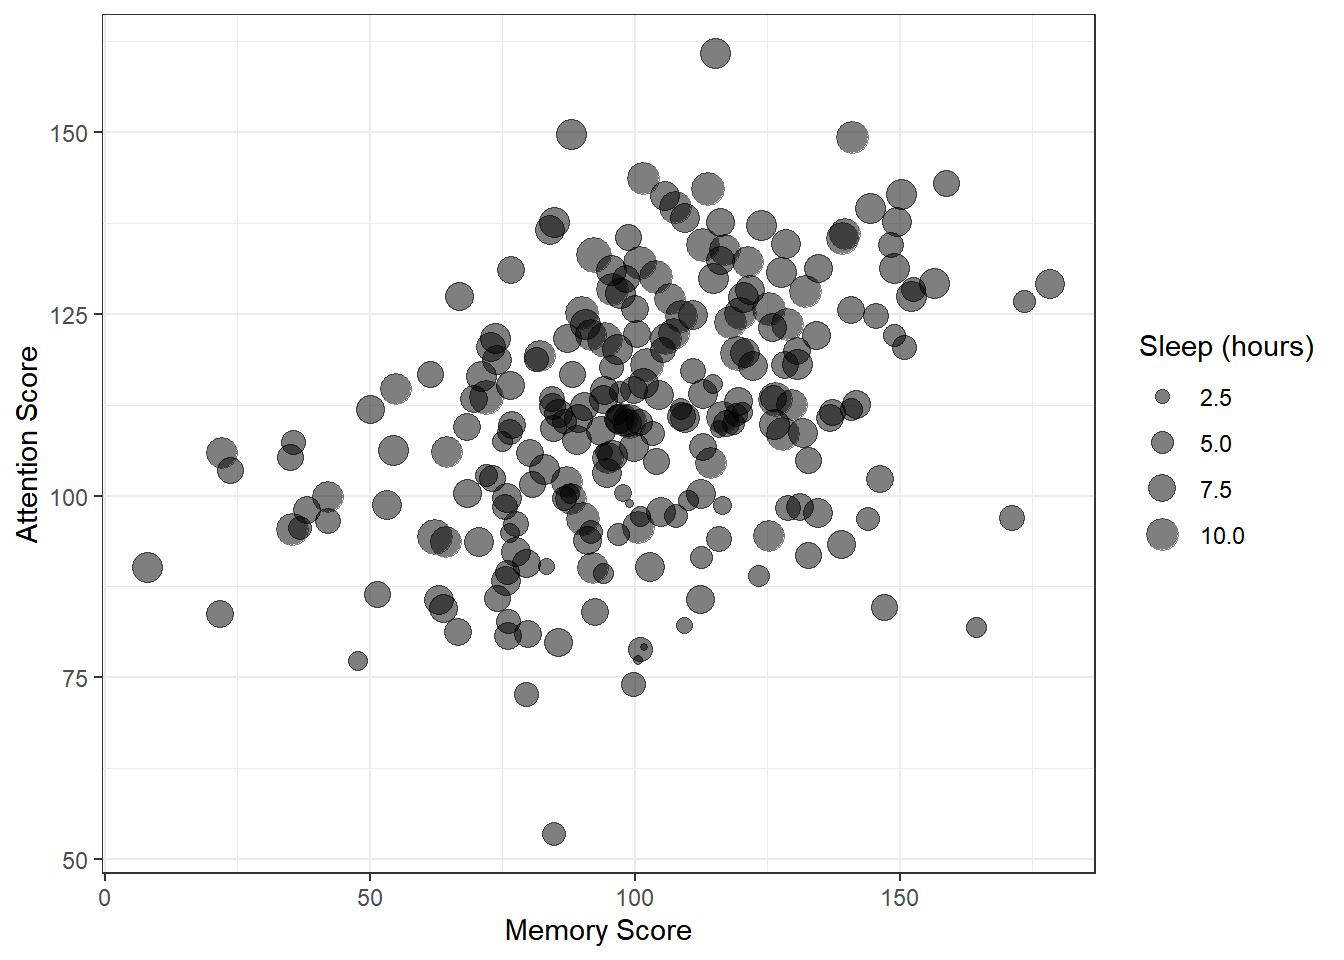
\includegraphics[width=1\linewidth]{05_multiple_regression_3_files/figure-latex/unnamed-chunk-19-1} 

}

\caption{TRUE}\label{fig:unnamed-chunk-19}
\end{figure}

\hfill\break
\hfill\break
\textbf{3.}

The researcher is interested to know whether annual consumption of blueberries has any bearing on \texttt{memory\_scores}, and so wants to add \texttt{blueberries} to the model in \texttt{memory2}.

\hfill\break
Determine the Bayes Factor comparing \texttt{memory2} with a model that additionally contains \texttt{blueberries}.

\begin{itemize}
\item
  The Bayes Factor for the model comparison is (to 2 decimal places)
\item
  The Bayes Factor indicates that the model with \texttt{blueberries} is more likelyless likely than the model without it.
\item
  Should the researcher add \texttt{blueberries} to the model? noyesif it tastes good
\end{itemize}

Try yourself first, then click for the code

\begin{Shaded}
\begin{Highlighting}[]
\CommentTok{\# add blueberries to memory2; store in memory3.BF}
\NormalTok{memory3.BF }\OtherTok{\textless{}{-}} \FunctionTok{lmBF}\NormalTok{(memory\_score }\SpecialCharTok{\textasciitilde{}}\NormalTok{ iq }\SpecialCharTok{+}\NormalTok{ age }\SpecialCharTok{+}\NormalTok{ attention }\SpecialCharTok{+}\NormalTok{ sleep }\SpecialCharTok{+}\NormalTok{ blueberries, }\AttributeTok{data =} \FunctionTok{as.data.frame}\NormalTok{(memory\_data) )}

\CommentTok{\# calculate the BF for memory3 vs memory2}
\NormalTok{memory3.BF }\SpecialCharTok{/}\NormalTok{ memory2.BF}
\SpecialCharTok{\textgreater{}}\NormalTok{ Bayes factor analysis}
\SpecialCharTok{\textgreater{}} \SpecialCharTok{{-}{-}{-}{-}{-}{-}{-}{-}{-}{-}{-}{-}{-}{-}}
\ErrorTok{\textgreater{}}\NormalTok{ [}\DecValTok{1}\NormalTok{] iq }\SpecialCharTok{+}\NormalTok{ age }\SpecialCharTok{+}\NormalTok{ attention }\SpecialCharTok{+}\NormalTok{ sleep }\SpecialCharTok{+}\NormalTok{ blueberries }\SpecialCharTok{:} \FloatTok{0.1663574}\NormalTok{ ±}\DecValTok{0}\NormalTok{\%}
\SpecialCharTok{\textgreater{}} 
\ErrorTok{\textgreater{}}\NormalTok{ Against denominator}\SpecialCharTok{:}
\ErrorTok{\textgreater{}}\NormalTok{   memory\_score }\SpecialCharTok{\textasciitilde{}}\NormalTok{ iq }\SpecialCharTok{+}\NormalTok{ age }\SpecialCharTok{+}\NormalTok{ attention }\SpecialCharTok{+}\NormalTok{ sleep }
\SpecialCharTok{\textgreater{}} \SpecialCharTok{{-}{-}{-}}
\ErrorTok{\textgreater{}}\NormalTok{ Bayes factor type}\SpecialCharTok{:}\NormalTok{ BFlinearModel, JZS}
\end{Highlighting}
\end{Shaded}

\end{exercise}

\hypertarget{summary-of-key-points-1}{%
\section{Summary of key points}\label{summary-of-key-points-1}}

\begin{itemize}
\item
  We can compare a model with one that has more predictors by using \texttt{anova(model1,\ model2)}.
\item
  We can compare models using Bayes Factors with \texttt{lmBF} in the \texttt{BayesFactor} package.
\item
  A \textbf{Bayes Factor} is probability of one model relative to another, \emph{given the data}.
\item
  To compare Bayes Factors of models:

  \begin{itemize}
  \item
    First obtain the Bayes Factors for \texttt{model1} and \texttt{model2}.
  \item
    Then use \texttt{model2\ /\ model1} to get the Bayes Factor, indicating how much more likely \texttt{model2} is.
  \end{itemize}
\item
  Bayes Factors less than 1 indicate evidence for \texttt{model1}
\item
  Bayes Factors greater than 1 indicate evidence for \texttt{model2}
\item
  We can report Bayes Factors as \(BF_{10}\) = 2.23 (or BF10 = 2.23)
\end{itemize}

\hfill\break

Next week's session will build on what was done in this session, so make sure you understand what was covered and ask if there's anything you're unsure of.

\hypertarget{anova-repeated-measures}{%
\chapter{ANOVA: Repeated measures}\label{anova-repeated-measures}}

\hypertarget{pre-post-data-effect-sizes-clinically-significant-change}{%
\chapter{Pre-post data, effect sizes, clinically significant change}\label{pre-post-data-effect-sizes-clinically-significant-change}}

\hypertarget{regression-assessment-2022}{%
\chapter{Regression Assessment 2022}\label{regression-assessment-2022}}

\hypertarget{regression-assessment-2022-faqs}{%
\chapter{Regression Assessment 2022: FAQs}\label{regression-assessment-2022-faqs}}

\hypertarget{appendix-appendices}{%
\appendix}


  \bibliography{book.bib,packages.bib}

\end{document}
